\documentclass[openright,twoside,10pt]{book}
\usepackage[b5paper,left=2cm,top=2.5cm,right=1.5cm,bottom=2.5cm]{geometry} 
\usepackage[spanish, es-tabla]{babel} % espanol
\usepackage[utf8]{inputenc} % acentos sin codigo
\usepackage{graphicx} % gráficos
\usepackage{lscape}
\usepackage{fancyvrb}
\usepackage{fancyhdr}
\usepackage{wrapfig}
\usepackage[hidelinks]{hyperref}
\usepackage{biblatex}
\renewcommand*{\bibfont}{\small}
\bibliography{bibliografia}
\usepackage{float}
\usepackage{libertine}
\usepackage{csquotes}
\makeatletter
\patchcmd{\@verbatim}
  {\verbatim@font}
  {\verbatim@font\small}
  {}{}
\makeatother


\providecommand{\tightlist}{%
  \setlength{\itemsep}{0pt}\setlength{\parskip}{0pt}}
  
\setlength{\parskip}{10pt plus 1pt minus 1pt}
 % aqui definimos el encabezado de las paginas pares e impares.
\rhead[]{}

\renewcommand{\headrulewidth}{0.5pt}

% aqui definimos el pie de pagina de las paginas pares e impares.
\rfoot[\thepage]{\thepage}
\cfoot[]{}
\renewcommand{\footrulewidth}{0pt}

%redefino el verbatim
%\renewenvironment{verbatim}{\begin{Verbatim}[frame=single,fontsize=\small]}{\end{Verbatim}}


% aqui definimos el encabezado y pie de pagina de la pagina inicial de un capitulo.
\fancypagestyle{plain}{
\fancyhead[R]{}
\fancyfoot[C]{}
\fancyfoot[R]{\thepage}
\renewcommand{\headrulewidth}{0.5pt}
\renewcommand{\footrulewidth}{0pt}
}

\pagestyle{fancy} % seleccionamos un estilo

\date{22 de junio de 2017}
\author{Julio Gracia Gutiérrez}
\title{Desarrollo de software educativo de apoyo a la docencia en la Teoría de
Conjuntos.}

\begin{document}
    {
        \fontfamily{phv}\selectfont
        \begin{titlepage}
        \begin{center}
            \vspace*{-1in}
            \begin{figure}[htb]
                \begin{center}
                    
\includegraphics[width=3cm]{./latex/img/logo}
                \end{center}
            \end{figure}
            \begin{Large}
                \textbf{Universidad de Valladolid}
            \end{Large}

            \vspace*{0.15in}
            \vspace*{0.6in}
            \begin{Huge}
                {Escuela de Ingeniería Informática\\}
            \end{Huge}
            \vspace*{0.2in}
            \begin{Large}
                \textbf{\textsc{Trabajo Fin de Grado\\}}
            \end{Large}
            \vspace*{0.5in}
            \begin{Large}
                { Grado en Ingeniería Informática}\\
                { Mención en INGENIERÍA DE SOFTWARE \\}
            \end{Large}
            \vspace*{0.5in}
            %\rule{140mm}{0.1mm}\\
            \vspace*{0.3in}
            \begin{large}
                \textbf{{\LARGE Desarrollo de software educativo de apoyo a la docencia en la Teoría de
Conjuntos.\\}}
            \end{large}
            \vspace*{0.3in}
            %\rule{140mm}{0.1mm}\\
            \vspace*{1.3in}
            \begin{large}
                \begin{flushright}
                    Autor:\\
                    \textbf{Julio Gracia Gutiérrez} \\
                    \vspace*{0.3in}
                    Tutor:\\
                    \textbf{María Felisa Pérez Martínez}
                \end{flushright}
            \end{large}
        \end{center}
    \end{titlepage}

    }
    
    \newpage
    \mbox{}	
    \thispagestyle{empty} % para que no se numere esta página

    \chapter*{}
    \pagenumbering{Roman} % para comenzar la numeración de paginas en números romanos

    \begin{flushright}
        \textit{%Dedicatoria,\\
        A los amigos, que siempre están ahí cuando los necesito.}
    \end{flushright}

    \chapter*{Agradecimientos} % si no queremos que añada la palabra "Capitulo"
    \addcontentsline{toc}{chapter}{Agradecimientos} % si queremos que aparezca en el índice
    \markboth{AGRADECIMIENTOS}{AGRADECIMIENTOS} % encabezado 

    \emph{``Si quieres ir rápido, camina solo; pero si quieres llegar lejos,
    camina acompañado''} (proverbio africano)
    
    En primer lugar, querría dar las gracias a la Escuela y a sus
    profesores, por guiarme de la mejor forma que han podido a lo largo de
    los años que he estado aquí. También dar las gracias a mi tutora Marisa
    por ser un apoyo constante a lo largo del TFG.
    
    Después, me gustaría dar las gracias a los miembros del GUI por ser
    amigos y constantes mentores, ayudándome y enseñándome cuando ha sido
    necesario.
    
    Por último, agradecer a Andrés, Guille, Jose, Isma, Lobo, Victor y
    Provecho por estar siempre ahí y conseguir que estos años sean
    inolvidables. No dudo de que si a día de hoy estoy escribiendo estas
    palabras se debe a su apoyo, comprensión y ayuda.

    \chapter*{Resumen} % si no queremos que añada la palabra "Capitulo"
    \addcontentsline{toc}{chapter}{Resumen} % si queremos que aparezca en el índice
    \markboth{RESUMEN}{RESUMEN} % encabezado
    %\begin{flushleft}

    En este Trabajo Fin de Grado se va a desarrollar un software de ayuda
    para la docencia de la asignatura ``Matemática Discreta'' del Grado en
    Ingeniería Informática de la Escuela de Ingeniería Informática de la
    Universidad de Valladolid.
    
    El objetivo del presente trabajo es desarrollar un prototipo funcional
    de una aplicación web orientada a mejorar el aprendizaje y afianzar el
    conocimiento de los contenidos relativos a la Teoría de Conjuntos
    impartidos en dicha asignatura.
    
    En este contexto será necesario plantear la arquitectura de la
    aplicación que se va a implementar. La solución escogida consiste en
    utilizar Angular programado en TypeScript para el front-end, Node.js
    programado en JavaScript y una base de datos relacional MariaDB para el
    back-end. Angular es una plataforma de desarrollo para aplicaciones web
    de TypeScript de código abierto. Node.js es un entorno en tiempo de
    ejecución multiplataforma asíncrono, de código abierto, para la capa del
    servidor. MariaDB es un sistema de gestión de bases de datos derivado de
    MySQL.

    %\end{flushleft}


    \chapter*{Abstract} % si no queremos que añada la palabra "Capitulo"
    \addcontentsline{toc}{chapter}{Abstract} % si queremos que aparezca en el índice
    \markboth{ABSTRACT}{ABSTRACT} % encabezado
  
    In the present thesis, a help software will be developed for the subject
    ``Discrete Mathematics'' in the Degree of Computer Science of the School
    of Computer Science of the University of Valladolid.
    
    The aim of this project is to develop a functional prototype of an
    online application, oriented to the improvement in both, the processes
    of learning and of reinforcement of the contents related to the set
    theory given in the subject mentioned above.
    
    At this stage, the contemplation of the application setting that is
    going to be implemented will be necessary. The chosen solution consists
    of using Angular, programmed in TypeScript for the front-end, Node.js
    programmed in JavaScript, and a relational MariaDB database for the
    back-end. Angular is a development platform for TypeScrip online
    open-source model applications. Node.js is an open-source,
    cross-platform, run-time environment for the server-side. MariaDB is a
    database management system derived from MySQL.

    \tableofcontents % indice de contenidos

    \cleardoublepage
    \addcontentsline{toc}{chapter}{Lista de figuras} % para que aparezca en el indice de contenidos
    \listoffigures % indice de figuras

    \cleardoublepage
    \addcontentsline{toc}{chapter}{Lista de tablas} % para que aparezca en el indice de contenidos
    \listoftables % indice de tablas

    \chapter{Introducción}
    
    \section{Descripción del problema}\label{descripciuxf3n-del-problema}
    
    \pagenumbering{arabic}
    
    Los alumnos que entran en el primer curso de una ingeniería experimentan
    grandes cambios a nivel académico. Esto es debido al uso de diferentes
    metodologías en la docencia y al aumento del volumen de contenidos tanto
    teóricos como prácticos en comparación con etapas anteriores. Algunas
    asignaturas parten de los conocimientos adquiridos durante los cursos de
    bachillerato pero otras tienen contenidos totalmente nuevos. La
    procedencia de los estudiantes es heterogénea (PAU y Módulos Superiores)
    y ,por tanto, habrán tenido diferente grado de contacto con los
    contenidos de la titulación. En particular, la asignatura
    \enquote{Matemática Discreta}, objeto de la aplicación desarrollada en
    este trabajo, incluye conceptos y resultados matemáticos que no han sido
    explorados con anterioridad.
    
    Para tener una buena base en informática es necesario conseguir un buena
    base matemática. En el primer año del grado, los estudiantes pueden
    experimentar una falta de motivación en asignaturas de este tipo debido
    a la complejidad de las mismas y a que no consiguen encontrar una
    aplicación práctica real, ni son conscientes de su importancia tanto
    para asignaturas futuras como para su vida profesional.
    
    La asignatura \enquote{Matemática Discreta} forma parte de las
    asignaturas de carácter básico del plan de estudios del Grado en
    Ingeniería Informática. Con ella se pretende ofrecer una formación
    básica y sólida al futuro ingeniero informático. Básica, en el sentido
    que los diferentes aspectos serán tratados a un nivel introductorio, y
    sólida, en el sentido de que los conocimientos adquiridos deben sentar
    las bases para desenvolverse en el resto de su formación académica y
    desarrollo profesional. Se trata de habilitar a los estudiantes para que
    adquieran las destrezas necesarias para seguir aprendiendo los aspectos
    de la Informática relacionados con la Lógica, Conjuntos, Relaciones y
    Combinatoria, que podrán aplicar en disciplinas como la Inteligencia
    Artificial, las Bases de Datos o la Estadística.
    
    \section{Objetivo}\label{objetivo}
    
    El objetivo final de este trabajo es proporcionar al alumno un
    complemento educativo en el estudio de la asignatura \enquote{Matemática
    Discreta} para el afianzamiento de algunos de los conocimientos que en
    ella se desarrollan. Para ello, se busca crear una plataforma que mejore
    la comunicación alumno-profesor y dote al profesor de herramientas que
    faciliten la distribución de los contenidos de la asignatura. La
    aplicación ha de facilitar al alumno el repaso de los conceptos teóricos
    más importantes de los temas relacionados con la Teoría de Conjuntos, la
    evaluación de su grado de aprendizaje a través de la realización de
    cuestionarios tipo test, así como el planteamiento de dudas al profesor.
    Además la aplicación recogerá estadísticas acerca de los conceptos
    consultados, dudas planteadas y test realizados por parte de los alumnos
    matriculados en la asignatura, que ayuden al profesor a detectar
    aquellos conceptos que representan mayor dificultad para el estudiante.
    
    \section{Contexto}\label{contexto}
    
    La metodología docente actual de la asignatura
    \cite{guiamatematicadiscreta} se basa en la combinación de sesiones
    teórico-prácticas en aula, sesiones prácticas en grupos reducidos y
    trabajo tanto grupal como individual. Concretamente se destinan 28 horas
    a las clases teórico-prácticas, 30 horas a las prácticas, 10 horas al
    estudio y trabajo grupal y 80 horas al estudio y trabajo individual. El
    presente trabajo se centra en este último apartado, ya que considero que
    es en el que el alumno puede sufrir mayores dificultades al no contar
    con la dirección del profesor ni con la ayuda de un grupo.
    
    El desarrollo de la asignatura consiste en clases magistrales
    participativas, en las que se imparten conceptos y técnicas que deben
    ser asimilados con las horas de estudio individual. Gracias al
    afianzamiento de estos contenidos, el alumno será capaz de participar de
    forma activa en las sesiones prácticas y teóricas, así como superar
    satisfactoriamente las diversas pruebas escritas que se realizan a lo
    largo del curso. Todo ello influye positivamente en la calificación.
    
    El material básico del que dispone el alumno es un documento pdf en el
    que se recogen los conceptos y resultados teóricos, ejemplos y
    ejercicios tipo que han de adquirirse para superar la asignatura.
    
    \section{Solución adoptada}\label{soluciuxf3n-adoptada}
    
    Debido al tamaño del temario y a su complejidad, el estudio de esta
    asignatura puede resultar difícil. Tampoco ayuda el formato del material
    básico, ya que es un documento PDF que no cuenta con ningún marcador.
    Esto dificulta enormemente la búsqueda de un concepto concreto, así como
    la relación entre conceptos, ya que las únicas herramientas con la que
    los alumnos cuentan para ello son las palabras claves que están
    resaltadas en negrita y la función de búsqueda de palabras del editor de
    PDF utilizado.
    
    Por otro lado, el procedimiento para plantear dudas requiere que el
    alumno se ponga en contacto con el profesor, ya sea presencialmente o
    mediante el correo electrónico, y el profesor resuelva la duda de manera
    individual. La duda, por tanto, será respondida únicamente a nivel
    personal, por lo que es complicado que el resto de alumnos se enteren de
    las dudas que han planteado sus compañeros y de las soluciones que el
    profesor ha dado a dichas dudas. A su vez, esto puede conllevar que el
    profesor resuelva varias veces la misma duda.
    
    Finalmente, es necesario algún sistema que permita al alumno saber de
    forma aproximada su nivel de preparación para ayudarle a afrontar las
    etapas finales de la asignatura.
    
    Lo que buscamos es una herramienta que nos permita localizar conceptos
    de forma rápida, entender las relaciones entre conceptos, reducir el
    tiempo malgastado tanto por parte del profesor como del alumno, evitando
    el planteamiento repetido de dudas ya resueltas con anterioridad y
    facilitando al alumno la resolución concreta de dudas y, por último,
    dotar al alumno de un mecanismo de comprobación de conocimientos
    adquiridos. Esta herramienta debe ser accesible por cualquier miembro de
    la comunidad educativa de la Universidad de Valladolid.
    
    \section{Estructura de la memoria}\label{estructura-de-la-memoria}
    
    En base al esquema seguido para la realización del presente trabajo, se
    ha estructurado la memoria de la misma manera:
    
    INTRODUCCIÓN: Se describe el porqué de este proyecto y los objetivos del
    mismo
    
    TECNOLOGÍAS UTILIZADAS: Contiene información sobre las tecnologías
    escogidas y explicación de ciertos conceptos clave para entenderlas.
    
    PLAN DE PROYECTO: En este capítulo se detalla la planificación del
    proyecto.
    
    DESARROLLO DEL PROYECTO: La parte fundamental del proyecto es el
    desarrollo de un prototipo de plataforma web. En este capítulo se
    profundizará en el proceso de desarrollo, que incluye las etapas de
    análisis, desarrollo y despliegue.
    
    CONCLUSIONES Y RESULTADOS: Tras realizar una serie de pruebas al
    prototipo, se presentarán las conclusiones y se analizarán los
    resultados así como posibles mejoras a tener en cuenta.
    
    \chapter{ Tecnologías utilizadas }
    
    \section{Definiciones previas
    necesarias}\label{definiciones-previas-necesarias}
    
    \begin{itemize}
    \item
      \textbf{JavaScript:} JavaScript (abreviado como JS) es un lenguaje
      multi-paradigma, ligero e interpretado. \cite{mozilla_javascript}
    \item
      \textbf{TypeScript:} TypeScript es un superconjunto de JavaScript que
      permite el uso de clases, interfaces y tipado estático. El uso de
      variables tipadas de TypeScript aporta mayor robustez al código.
      \cite{enriqueoriol2017, stackoverflow_Typescript}
    \item
      \textbf{ECMAScript:} ECMAScript (abreviado como ES) es un lenguaje de
      scripting que forma la base de JavaScript. Está recogido en los
      estándares ECMA-262 y ECMA-402 de ECMA International. Al referirnos a
      ES5 nos referimos a la quinta versión del estándar ECMA-262, mientras
      que al hablar de ES2015 o ES6 nos referimos al estándar ECMA-262 en su
      sexta versión. Actualmente los navegadores soportan ES5, por lo
      cualquier lenguaje derivado de ECMAScript(como son JavaScript y
      TypeScript) deben de ser traspilado a ES5. \cite{mozilla_ecmascript}
    \item
      \textbf{Transpilar:} Transpilar es un término relativamente nuevo,
      proviene del inglés \emph{transpiler}, fruto de la unión de las
      palabras \emph{translate} y \emph{compiler}. Es la operación de
      traducción de un lenguaje a otro, siendo ambos del mismo nivel de
      abstracción aproxiamadamente.
      \cite{enriquefernandezguerra_typescript, builtbyedgar_transpilar}
    \item
      \textbf{Gestor de paquetes:} Un gestor de paquetes mantiene un
      registro del software que está instalado en su ordenador, y le permite
      instalar software nuevo, actualizarlo a versiones más recientes, o
      eliminar software de una manera sencilla. Como su propio nombre
      sugiere, los gestores de paquetes gestionan paquetes: conjuntos de
      ficheros que se agrupan y que puede instalar y eliminar como conjunto.
      La labor de un gestor de paquetes es la de presentar una interfaz que
      asista al usuario en la tarea de administrar el conjunto de paquetes
      que están instalados en su sistema. \cite{debian_gestorpaquetes}
    \item
      \textbf{Plataforma:} Una plataforma es un sistema que engloba los
      componentes, interfaces y librerías necesarios para permitir a los
      desarrolladores compilar, ejecutar y depurar sus aplicaciones.
    \item
      \textbf{Framework:} Desde el punto de vista del desarrollo de
      software, un framework es una estructura de soporte definida, en la
      cual otro proyecto de software puede ser organizado y desarrollado.
    \item
      \textbf{Open source:} La terminología open source incluye a aquellos
      softwares que cumplen los siguientes requisitos
      \cite{opensource_definition} :
    
      \begin{itemize}
      \tightlist
      \item
        \textbf{Distribución libre:}La licencia no restringirá a ninguna de
        las partes vender o regalar el software como un componente de un
        conjunto de software.
      \item
        \textbf{Código fuente:} El programa debe incluir el código fuente
        sin ofuscar o dotar de un mecanismo para conseguirlo,
        preferentemente de forma gratuita mediante una descarga online.
      \item
        \textbf{Trabajos derivados:} La licencia debe permitir
        modificaciones y trabajos derivados, y permitir que se distribuyan
        de forma libre.
      \item
        \textbf{Integridad del código fuente del autor:} La licencia podría
        permitir no distribuir el código fuente del programa modificado si
        permite la distribución de parches. La licencia debe permitir
        explícitamente la distribución del software construido a partir de
        las fuentes modificadas.
      \item
        \textbf{Sin discriminación:} La licencia no debe discriminar a
        ninguna persona ni colectivo.
      \item
        \textbf{Para todos los ámbitos:} La licencia no debe restringir el
        uso en función del ámbito para el que se vaya a utilizar el
        software.
      \item
        \textbf{Distribución de licencia:} Los derechos asociados al
        software deben aplicarse a todos los programas redistribuidos.
      \item
        \textbf{La licencia no debe estar asociada a un producto:} Los
        derechos del software no deben depender del paquete de software en
        el que se distribuya
      \item
        \textbf{La licencia no debe restringir a otros programas que se
        distribuyan junto a ella.}
      \item
        \textbf{La licencia debe ser independiente de la tecnología
        utilizada.}
      \end{itemize}
    \item
      \textbf{Back-end:} Término técnico para la capa de acceso a datos.
    \item
      \textbf{Front-end:} Término técnico para la capa de presentación de
      una aplicación. Concierne los componentes externos del sitio o
      aplicación web.
    \item
      \textbf{Propiedad:} \cite{mozilla_properties} Una propiedad de un
      objeto puede ser explicada como una variable que se adjunta al objeto.
      Las propiedades de un objeto definen las características de un objeto.
      Un valor de propiedad puede ser una función, la cual es conocida
      entonces como un método del objeto.
    \item
      \textbf{Licencia GPL:} \cite{GNU_GPL, GNU_copyleft} La licencia GPL o
      GNU GPL es una licencia copyleft. Esto es, un método general que
      requiere que todas las versiones modificadas y extendidas sean también
      libres.
    \item
      \textbf{API:} API significa interfaz de programación de aplicaciones
      (Application Programming Interface). Las APIs ofrecen una forma de
      estándar de dotar de funcionalidad a una aplicación, definiendo que
      funciones y métodos son accesibles.
    \end{itemize}
    
    \section{Node.js}\label{node.js}
    
    \begin{figure}[H]
        \begin{center}
            
\includegraphics[scale=0.05]{img/nodejs.png}
        \end{center}
        \caption{Logo de Node.js}
    \end{figure}
    
    Node.js es un entorno de ejecución para JavaScript construido con el
    motor de JavaScript V8 de Chrome
    
    \subsection{Instalación}\label{instalaciuxf3n}
    
    Para instalar node vamos a usar nvm. En este proyecto utilizaremos la
    versión \textbf{6.9.5}
    
    \begin{verbatim}
    curl -sL \
    https://raw.githubusercontent.com/creationix/nvm/v0.32.0/install.sh \
    -o install_nvm.sh
    bash install_nvm.sh
    export NVM_DIR="/root/.nvm"
    [ -s "$NVM_DIR/nvm.sh" ] && . "$NVM_DIR/nvm.sh"
    \end{verbatim}
    
    En este proyecto usaremos la versión \textbf{6.9.5}
    
    \begin{verbatim}
    nvm install v6.9.5
    \end{verbatim}
    
    \newpage
    
    \section{NPM}\label{npm}
    
    \begin{figure}[H]
        \begin{center}
            
\includegraphics[scale=0.8]{img/npm.png}
        \end{center}
        \caption{Logo de NPM}
    \end{figure}
    
    Npm es un gestor de paquetes que permite a los desarrolladores de
    JavaScript compartir y reutilizar código. Gracias a este gestor podemos
    conseguir de forma sencilla y actualizada las dependencias que va a
    tener nuestra aplicación. Este gestor de paquetes resulta esencial, ya
    que de él dependen Angular, Angular CLI y Node.js.
    
    \subsection{Instalación:}\label{instalaciuxf3n-1}
    
    NPM es instalado junto con Node.js en el apartado anterior. Vamos a
    actualizarlo.
    
    \begin{verbatim}
    npm install -g npm
    \end{verbatim}
    
    \subsection{Principales comandos
    utilizados:}\label{principales-comandos-utilizados}
    
    \begin{itemize}
    \item
      \texttt{npm\ install}
    
      Este comando instala todas las dependencias que hayamos declarado en
      nuestro fichero de configuración.En caso de especificar un nombre al
      final del comando instalaremos únicamente la dependencia nombrada.
      Este comando instala los paquetes elegidos, así como todos los
      paquetes de los que estos dependa. Usualmente se usará la opción
      --save que nos guarda la dependencia en nuestro fichero de
      configuración, de forma que podamos instalarla posteriormente
    \item
      \texttt{npm\ uninstall\ {[}nombre{]}}
    
      Este comando elimina la dependencia nombrada de nuestro sistema.
      Usualmente, se usará la opción --save para eliminarla también del
      fichero de configuración.
    \end{itemize}
    
    \section{Express}\label{express}
    
    \begin{figure}[H]
        \begin{center}
            
\includegraphics[scale=0.3]{img/express.png}
        \end{center}
        \caption{Logo de Express}
    \end{figure}
    
    Express es un framework de desarrollo de aplicaciones web y APIs para
    Node.js
    
    \subsection{Instalación}\label{instalaciuxf3n-2}
    
    \begin{verbatim}
    npm install express
    \end{verbatim}
    
    \subsection{Principales utilidades}\label{principales-utilidades}
    
    Nos facilita el manejo de:
    
    \begin{itemize}
    \tightlist
    \item
      \textbf{Estáticos:} Ruta pública donde generalmente se alojan assets
      (CSS, imágenes, JS).
    \end{itemize}
    
    \begin{verbatim}
    app.use(express.static(path.join(__dirname, 'public')));
    \end{verbatim}
    
    \begin{itemize}
    \tightlist
    \item
      \textbf{Controladores:} Encargados de controlar las peticiones http.
    \end{itemize}
    
    \begin{verbatim}
    app.post('/login', function(req, res) {});
    \end{verbatim}
    
    \begin{itemize}
    \tightlist
    \item
      \textbf{Sesiones y cookies:}
    \end{itemize}
    
    \begin{verbatim}
    app.use(express.cookieParser('your secret here'));
    app.use(express.session());
    \end{verbatim}
    
    \section{Angular}\label{angular}
    
    \begin{figure}[H]
        \begin{center}
            
\includegraphics[scale=0.6]{img/angular.png}
        \end{center}
        \caption{Logo de angular}
    \end{figure}
    
    Angular es una plataforma open source de desarrollo de front-end
    desarrollado por Google. Está basado en componentes, que es una
    combinación de una plantilla HTML con un controlador.
    
    Si bien está desarrollado con Javascript y permite el desarrollo con ES5
    o superior, la comunidad de desarrolladores(incluyendo los responsables
    del proyecto de Google) prefiere utilizar TypeScript.
    \cite{angular_docs}
    
    \begin{figure}[H]
        \begin{center}
            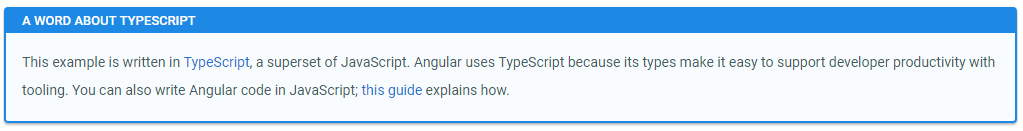
\includegraphics[width=\textwidth]{img/aboutTypescript.png}
        \end{center}
        \caption{Google sobre TypeScript}
    \end{figure}
    
    \subsection{¿Qué es un controlador?}\label{quuxe9-es-un-controlador}
    
    \begin{verbatim}
    @Component({
        selector: ‘my-app’,
        template: <h1>Hello {{name}}</h1>
    })
    \end{verbatim}
    
    Todos los componentes inician con el decorador \textcite{Component} que
    describe cómo se comporta el componente. Entre otras opciones, define
    como incluir el componente en una página HTML, mediante la propiedad
    selector; y como está estructurado visualmente mediante la propiedad
    template. En el ejemplo dado, si quisiéramos utilizar el componente en
    una página HTML se usaría el elemento
    \texttt{\textless{}my-app\textgreater{}}, y el componente se ve como la
    frase \enquote{Hello \{\{name\}\}} dentro de un elemento de de título 1.
    
    En un desarrollo de mayor tamaño en lugar de definir la plantilla HTML
    en el propio componente, se usará la propiedad \texttt{templateUrl} para
    definir dónde buscar la plantilla HTML. De igual forma, se separarían
    los códigos CSS mediante la propiedad \texttt{styleUrls}. Ejemplo:
    
    \begin{verbatim}
    @Component({
        selector: ‘my-app’,    
        templateUrl: 'nombre_del_archivo.html',
        styleUrls: ['nombre_del_archivo1.css', 'nombre_del_archivo2.css']
    })
    \end{verbatim}
    
    Siguiendo la trayectoria de AngularJs, precursor del actual Angular,
    conseguimos acceder a las propiedades del controlador mediante el uso de
    \{\{ nombre\_variable \}\}. En este caso accederíamos a la propiedad
    \texttt{name}.
    
    \begin{verbatim}
    export class AppComponent { name = ‘Angular’; }
    \end{verbatim}
    
    Define la clase del controlador. En el caso de ejemplo, el controlador
    solo tiene la propiedad name, que contiene la cadena de texto
    \enquote{Angular}
    
    \newpage
    
    \section{Angular CLI}\label{angular-cli}
    
    \begin{figure}[H]
        \begin{center}
            
\includegraphics[scale=0.3]{img/angular-cli.png}
        \end{center}
        \caption{Logo de angular-cli}
    \end{figure}
    
    Angular CLI es una herramienta utilizada para inicializar aplicaciones
    Angular, desarrollar componentes y para tareas de mantenimiento
    asociadas a ello. \cite{angular_cli}
    
    \subsection{Instalacion:}\label{instalacion}
    
    \begin{verbatim}
    npm install -g @angular/cli
    \end{verbatim}
    
    \subsection{Comandos relevantes
    utilizados:}\label{comandos-relevantes-utilizados}
    
    \begin{itemize}
    \item
      \texttt{ng\ new\ {[}nombre{]}}
    
      Inicializa una nueva aplicación Angular con el nombre elegido.
    \item
      \texttt{ng\ serve}
    
      Transpila la aplicación y monta un servidor web.
    \item
      \texttt{ng\ generate\ class\ {[}nombre{]}}
    
      Genera una clase con el nombre escogido. Una clase es una construcción
      que permite crear tipos personalizados mediante la agrupación de
      variables de otras clases y comportamientos comunes.
    \item
      \texttt{ng\ generate\ component\ {[}nombre{]}}
    
      Genera un componente con el nombre escogido.
    \item
      \texttt{ng\ generate\ service\ {[}nombre{]}}
    
      Genera un servicio con el nombre escogido. Un servicio es una función,
      con sus propiedades y métodos que puede ser incluida, mediante
      inyección de dependencias, en los componentes. Gracias a esto, se
      pueden desarrollar funciones para tareas específicas, como es la
      comunicación con el servidor. Permite reutilizar las funciones de
      forma rápida entre componentes, así como acceder a variables
      compartidas entre ellos.
    \end{itemize}
    
    \section{Bootstrap 4}\label{bootstrap-4}
    
    \begin{figure}[H]
        \begin{center}
            
\includegraphics[scale=0.15]{img/bootstrap4.png}
        \end{center}
        \caption{Logo de Bootstrap 4}
    \end{figure}
    
    Bootstrap es un framework de HTML, CSS y JavaScript para el desarrollo
    de front-end. En su versión 4 incluye componentes de angular que
    utilizaremos en el presente proyecto.
    
    \subsection{Instalación}\label{instalaciuxf3n-3}
    
    \texttt{npm\ install\ bootstrap@4.0.0-alpha.6}
    
    \newpage
    
    \section{MariaDB}\label{mariadb}
    
    \begin{figure}[H]
        \begin{center}
            
\includegraphics[scale=0.75]{img/mariadb.png}
        \end{center}
        \caption{Logo de MariaDB}
    \end{figure}
    
    MariaDB es un sistema de gestión de bases de datos derivado de MySQL con
    licencia GPL (General Public License). Está desarrollado por Michael
    Widenius (fundador de MySQL) y la comunidad de desarrolladores de
    software libre. Surgío a partir de la compra de Sun Microsystems por
    parte de Oracle para asegurar la existencia de una versión de MySQL con
    licencia GPL.
    
    \subsection{Instalación}\label{instalaciuxf3n-4}
    
    \begin{verbatim}
    sudo apt-get install software-properties-common
    sudo apt-key adv --recv-keys --keyserver\
     keyserver.ubuntu.com 0xF1656F24C74CD1D8
    sudo add-apt-repository 'deb [arch=amd64]\
     http://tedeco.fi.upm.es/mirror/mariadb/repo/10.2/debian\
     stretch main'
    sudo apt-get update
    sudo apt-get install mariadb-server
    \end{verbatim}
    
    \subsection{Ventajas y deventajas de MariaDB frente
    MySQL}\label{ventajas-y-deventajas-de-mariadb-frente-mysql}
    
    \begin{itemize}
    \item
      \textbf{Ventajas:}
      \cite{zeokat_mariadb, andergonzalez_mariadb, alidavergara_mariadb}
    
      \begin{itemize}
      \item
        \textbf{Nuevos motores de almacenamiento más eficientes:}
    
        Aria y XtraDB vienen a reemplazar a MyISAM e InnoDB respectivamente.
        Cabe destacar el mayor rendimiento de Aria, cuando recibe consultas
        complejas y tiene que realizar tablas temporales, éstas se cachean
        en memoria en vez de escribirlas en disco.
      \item
        \textbf{Estadísticas para índices y tablas:}
    
        Esto puede ayudar para la optimización de la base de datos. Se
        añaden nuevas tablas de sistema para recoger esta información.
      \item
        \textbf{Mejoras en el rendimiento y la eficiencia con respecto a
        MySQL:}
    
        Un ejemplo de esto es la eliminación o mejora de algunas
        conversiones no necesarias respecto a los juegos de caracteres.
      \item
        \textbf{Software libre:}
    
        MariaDB está respaldada por la comunidad de software libre.
      \end{itemize}
    \item
      \textbf{Desventajas:}
    
      \begin{itemize}
      \item
        \textbf{Coste migratorio:}
    
        En líneas generales, MySQL está más extendido, por lo que utilizar
        MariaDB suele acarrear un coste migratorio de los datos. Sin
        embargo, MariaDB asegura tener total compatibilidad. En este
        proyecto no nos afectará en absoluto.
      \end{itemize}
    \end{itemize}
    
    \chapter{ Plan del proyecto }
    
    El plan de desarrollo software es el documento que dirige la gestión de
    un proyecto software. Define las funciones técnicas y de gestión de
    proyectos, actividades y tareas necesarias para satisfacer los
    requisitos del proyecto. La finalidad de esta sección es conocer los
    puntos básicos de los que consta el proyecto, proporcionar los
    fundamentos en los que se basa y transmitir los aspectos básicos tal y
    como han sido entendidos y formulados. A continuación se describirá la
    visión general del proyecto donde se detalla su propósito, alcance y
    objetivos y la gestión del proceso donde se explica el coste estimado y
    la planificación de las fases principales e hitos del proyecto.
    
    \section{Vision general}\label{vision-general}
    
    \subsection{Propósito, alcance y
    objetivos}\label{propuxf3sito-alcance-y-objetivos}
    
    El objetivo del presente proyecto es desarrollar un prototipo de
    aplicación que sirva de apoyo para la asignatura de Matemática Discreta.
    La aplicación será un complemento educativo que permitirá al alumno
    repasar los conceptos teóricos más importantes, evaluar sus
    conocimientos mediante unos cuestionarios de tipo test y realizar
    consultas al profesor. Por parte del profesor permitirá introducir
    contenidos teóricos, resolver dudas, plantear preguntas para formar los
    cuestionarios y monitorizar el desempeño de los alumnos en la misma.
    
    Toda esta información aparecerá de manera detallada en el apartado
    Análisis de Requisitos del siguiente capítulo
    
    \subsection{Metodología utilizada}\label{metodologuxeda-utilizada}
    
    Se ha utilizado la metodología Kanban. Esta técnica se creó en Toyota, y
    se utiliza para controlar el avance del trabajo, en el contexto de una
    línea de producción. Los pricipios que rigen la metodología son los
    siguientes:
    
    \begin{itemize}
    \item
      \textbf{Calidad garantizada:} Todo lo que se hace debe salir bien a la
      primera, no hay margen de error. De aquí a que en Kanban no se premie
      la rapidez, sino la calidad final de las tareas realizadas. Esto se
      basa en el hecho que muchas veces cuesta más arreglarlo después que
      hacerlo bien a la primera.
    \item
      \textbf{Reducción del desperdicio:} Kanban se basa en hacer solamente
      lo justo y necesario, pero hacerlo bien. Esto supone la reducción de
      todo aquello que es superficial o secundario
    \item
      \textbf{Flexibilidad:} Lo siguiente a realizar se decide del backlog
      (o tareas pendientes acumuladas), pudiéndose priorizar aquellas tareas
      entrantes según las necesidades del momento
    \end{itemize}
    
    Para su implementación se ha utilizado la herramienta provista por
    Github usando las siguientes columnas:
    
    \begin{itemize}
    \item
      \textbf{To Do:} El backlog de tareas
    \item
      \textbf{In Progress:} Las tareas que se estan haciendo actualmente
    \item
      \textbf{Done:} Las tareas ya realizadas
    \end{itemize}
    
    \subsection{Evolución del plan}\label{evoluciuxf3n-del-plan}
    
    El presente documento se revisará a lo largo del Trabajo de Fin de Grado
    y se irá actualizando conforme a los cambios que surjan.
    
    \section{Gestión del proceso}\label{gestiuxf3n-del-proceso}
    
    \subsection{Estimación}\label{estimaciuxf3n}
    
    Se considerará que la dedicación media al proyecto será de un total de 4
    horas diarias con un solo recurso sin días de descanso. La fecha de
    inicio del proyecto es el 10/03/2017. Tras el estudio del plan de
    trabajo se estima que se requeriran aproximadamente 500 horas, por lo
    que se marca el hito de entrega del proyecto el 12/7/2017.
    
    \subsection{Plan de trabajo}\label{plan-de-trabajo}
    
    \begin{itemize}
    \tightlist
    \item
      \textbf{Reunión con el cliente y documentación}
    
      \begin{itemize}
      \tightlist
      \item
        Recopilar información sobre el objetivo que persigue el cliente
        mediante entrevistas personalizadas, así como estudio de la
        documentación que este nos facilite.
      \item
        \textbf{Duración:} 7 días
      \end{itemize}
    \item
      \textbf{Elicitación de requisitos}
    
      \begin{itemize}
      \tightlist
      \item
        Asegurar los requisitos extraidos de las entrevistas previas
        mediante la confirmación con el cliente. Este proceso se repetirá
        hasta conseguir extraer todos los requisitos que el cliente busca.
      \item
        \textbf{Duración:} 7 días
      \end{itemize}
    \item
      \textbf{Realización del diagrama de casos de uso y elaboración de un
      plan de trabajo provisional}
    
      \begin{itemize}
      \tightlist
      \item
        Realización de un plan de trabajo provisional para tener una marco
        de referencia a la hora de distribuir el tiempo. Para ello, se
        decidiran cuales son los casos de uso y se hara el diagrama
        correspondiente, sin profundizar.
      \item
        \textbf{Duración:} 2 días
      \end{itemize}
    \item
      \textbf{Diseño de las vistas de la aplicación y elicitación con el
      cliente}
    
      \begin{itemize}
      \tightlist
      \item
        Diseño en papel de las vistas de la aplicación.
      \item
        \textbf{Duración estimada:} 7 días
      \item
        \textbf{Duración real:} 7 días
      \end{itemize}
    \item
      \textbf{Estudio de las tecnologías actuales que nos permitan
      desarrollar el proyecto}
    
      \begin{itemize}
      \tightlist
      \item
        Estudio y comparación de las tecnologías actuales, su grado de
        adecuación al proyecto y su complejidad técnica, teniendo en cuenta
        los conocimientos previos de los que partimos.
      \item
        \textbf{Duración estimada:} 2 días
      \item
        \textbf{Duración real:} 2 días
      \end{itemize}
    \item
      \textbf{Aprendizaje y práctica de las tecnologías escogidas}
    
      \begin{itemize}
      \tightlist
      \item
        Realización de ejemplos sencillos para comprobar de forma práctica
        los datos recopilados en el punto anterior.
      \item
        \textbf{Duración estimada:} 2 días
      \item
        \textbf{Duración real:} 2 días
      \end{itemize}
    \item
      \textbf{Realización del plan de trabajo y estudio de los riesgos}
    
      \begin{itemize}
      \tightlist
      \item
        Basándonos en los conocimientos y destrezas adquiridos en el
        apartado anterior y en el plan provisional realizado con
        anterioridad, estudiar de los posibles riesgos y realizar planes de
        actuación para el caso de que se realicen. A mayores, se realiza un
        plan de trabajo de carácter definitivo.
      \item
        \textbf{Duración estimada:} 2 días
      \item
        \textbf{Duración real:} 2 días
      \end{itemize}
    \item
      \textbf{Realizacion de la descripcion en detalle de los casos de uso}
    
      \begin{itemize}
      \tightlist
      \item
        Basándonos en el diagrama realizado en el pasos anteriores,
        profundizamos en cada uno de los casos de uso, definiendo su
        descripción en detalle.
      \item
        \textbf{Duración estimada:} 4 días
      \item
        \textbf{Duración real:} 4 días
      \end{itemize}
    \item
      \textbf{Modelo de dominio y análisis de la base de datos}
    
      \begin{itemize}
      \tightlist
      \item
        Se definirá el modelo de dominio de la aplicación y se diseñará la
        base de datos basándonos en el.
      \item
        \textbf{Duración estimada:} 2 días
      \item
        \textbf{Duración real:} 2 días
      \end{itemize}
    \item
      \textbf{Realización básica de backend}
    
      \begin{itemize}
      \tightlist
      \item
        Programación de los elementos básicos y comunes a las aplicaciones
        Nodejs
      \item
        \textbf{Duración estimada:} 4 días
      \item
        \textbf{Duración real:} 4 días
      \end{itemize}
    \item
      \textbf{Realización de las funcionalidades relacionadas con las
      sesiones}
    
      \begin{itemize}
      \tightlist
      \item
        Realización en profundidad del diseño relacionado con las
        funcionalidades y programación del frontend y el backend de las
        funcionalidades relacionadas con las sesiones, esto es, permitir al
        usuario acceder a la aplicación, que se muestre de forma distinta
        para alumnos y profesores y permitir al usuario salir de la
        aplicación
      \item
        \textbf{Duracion estimada:} 12 días
      \item
        \textbf{Duracion real:} 10 días
      \end{itemize}
    \item
      \textbf{Realización de las funcionalidades relacionada con teoría}
    
      \begin{itemize}
      \tightlist
      \item
        Realización en profundidad del diseño de las funcionalidades y
        programación del frontend y el backend de las funcionalidades
        relacionadas con la teoria, esto es, mostrar la teoria organizada
        por temas, permitir la busqueda de teoría por concepto y permitir al
        profesor añadir y editar conceptos.
      \item
        \textbf{Duracion estimada:} 15 días
      \item
        \textbf{Duracion real:} 20 días
      \end{itemize}
    \item
      \textbf{Realización de las funcionalidades relacionadas con dudas}
    
      \begin{itemize}
      \tightlist
      \item
        Realización en profundidad del diseño de las funcionalidades y
        programación del frontend y el backend de las funcionalidades
        relacionadas con dudas, esto es, permitir al usuario ver las dudas
        ya preguntadas con anterioridad organizadas por conceptos, permitir
        generar nuevas dudas y permitir al profesor ver las dudas no
        resueltas y gestionarlas, ya sea reportándolas, ignorándolas o
        respondiéndolas.
      \item
        \textbf{Duracion estimada:} 15 días
      \item
        \textbf{Duracion real:} 19 días
      \end{itemize}
    \item
      \textbf{Realización de las funcionalidades relacionadas con
      cuestiones}
    
      \begin{itemize}
      \tightlist
      \item
        Realización en profundidad del diseño de las funcionalidades y
        programación del frontend y el backend de las funcionalidades
        relacionadas con cuestiones, esto es, permitir al alumno generar
        cuestionarios segun una serie de parámetros, resolverlos y conocer
        su resultado y permitir al profesor añadir y editar preguntas.
      \item
        \textbf{Duracion estimada:} 15 días
      \item
        \textbf{Duracion real:} 18 días
      \end{itemize}
    \item
      \textbf{Realización de las funcionalidades relacionadas con
      estadisticas}
    
      \begin{itemize}
      \tightlist
      \item
        Realización en profundidad del diseño de las funcionalidades y
        programación del frontend y el backend de las funcionalidades
        relacionadas con cuestiones, esto es, permitir al alumno generar
        cuestionarios segun una serie de parámetros, resolverlos y conocer
        su resultado y permitir al profesor añadir y editar preguntas.
      \item
        \textbf{Duracion estimada:} 3 días
      \item
        \textbf{Duracion real:} 3 días
      \end{itemize}
    \item
      \textbf{Realización de las funcionalidades relacionadas con
      herramientas}
    
      \begin{itemize}
      \tightlist
      \item
        Realización en profundidad del diseño de las funcionalidades y
        programación del frontend y el backend de las funcionalidades
        relacionadas con herramientas que permitan poner en práctica los
        conocimientos de la asignatura.
      \item
        \textbf{Duracion estimada:} 10 días
      \item
        \textbf{Duracion real:} No realizado
      \item
        \textbf{Motivo:} Las funcionalidades relacionadas con herramientas
        no fueron implementadas ya que, debido a una mala estimación de las
        funcionalidades anteriores, se descartó para cumplir el plazo de
        entrega.
      \end{itemize}
    \item
      \textbf{Mejora de la interfaz}
    
      \begin{itemize}
      \tightlist
      \item
        Realización de una interfaz mas allá de la interfaz útil.
      \item
        \textbf{Duracion estimada:} 4 días
      \item
        \textbf{Duracion real:} 3 días
      \end{itemize}
    \item
      \textbf{Realización de documentación del TFG}
    
      \begin{itemize}
      \tightlist
      \item
        Realización del presente documento, esto incluye los capítulos
        Introduccion y Conclusiones y los anexos Manual de usuario y Manual
        de instalación, así como la maquetación del resto de capítulos.
      \item
        \textbf{Duracion estimada:} 7 días
      \item
        \textbf{Duracion real:} 9 días
      \end{itemize}
    \item
      \textbf{Mejora de la interfaz}
    
      \begin{itemize}
      \tightlist
      \item
        Mejorar el aspecto de la aplicación
      \item
        \textbf{Duracion estimada:} 9 días
      \item
        \textbf{Duracion real:} No realizado
      \item
        \textbf{Motivo:} La mejora de la interfaz no fuer implementadas ya
        que, debido a una mala estimación de las funcionalidades anteriores,
        se descartó para cumplir el plazo de entrega.
      \end{itemize}
    \end{itemize}
    
    \newpage
    
    \subsection{Plan de Gestión de
    Riesgos}\label{plan-de-gestiuxf3n-de-riesgos}
    
    La lista de riesgos expuesta a continuación tiene las siguientes
    características:
    
    \begin{itemize}
    \item
      \textbf{Impacto}: Los riesgos serán catalogados del 1 al 5, siendo 1
      el riesgo menos peligroso y 5 el el riesgo más peligroso.
    \item
      \textbf{Probabilidad}: Los riesgos serán catalogados del 1 al 5,
      siendo 1 un riesgo muy poco probable y 5 un riesgo muy frecuente.
    \item
      \textbf{Plan de protección}: Plan para evitar o minimizar la
      probabilidad.
    \item
      \textbf{Plan de contingencia}: Plan de solución para minimizar el
      impacto.
    \end{itemize}
    
    \subsubsection{Riesgos}\label{riesgos}
    
    \begin{itemize}
    \tightlist
    \item
      \textbf{R-01 - Borrado de datos}
    
      \begin{itemize}
      \tightlist
      \item
        \textbf{Impacto:} 5
      \item
        \textbf{Probabilidad:} 2
      \item
        \textbf{Plan de protección:} Utilizar un sistema de control de
        versiones
      \item
        \textbf{Plan de contingencia:} Restaurar la última versión
      \end{itemize}
    \item
      \textbf{R-02 - Máquina personal averiada}
    
      \begin{itemize}
      \tightlist
      \item
        \textbf{Impacto:} El impacto se determinará en función del nivel de
        avería
      \item
        \textbf{Probabilidad:} 1
      \item
        \textbf{Plan de potección:} No hay
      \item
        \textbf{Plan de contingencia:} En función del nivel de avería se
        detallan 3 posibles planes:
    
        \begin{itemize}
        \tightlist
        \item
          \textbf{Nivel bajo (Impacto 2):} Intentar arreglar la máquina
        \item
          \textbf{Nivel medio (Impacto 3):} Intentar rescatar los datos
        \item
          \textbf{Nivel alto (Impacto 5):} Restaurar la última versión en
          otra máquina y continuar el proyecto desde esta.
        \end{itemize}
      \end{itemize}
    \item
      \textbf{R-03 - Enfermedad no banal}
    
      \begin{itemize}
      \tightlist
      \item
        \textbf{Impacto:} 5
      \item
        \textbf{Probabilidad:} 1
      \item
        \textbf{Plan de protección:} No hay
      \item
        \textbf{Plan de contingencia:} Replanificar teniendo en cuenta el
        tiempo disponible
      \end{itemize}
    \item
      \textbf{R-04 - Fallo de software de terceros}
    
      \begin{itemize}
      \tightlist
      \item
        \textbf{Impacto:} 4
      \item
        \textbf{Probabilidad:} 3
      \item
        \textbf{Plan de protección:} Ninguno
      \item
        \textbf{Plan de contingencia:} Se seguirán los siguientes pasos:
    
        \begin{enumerate}
        \def\labelenumi{\arabic{enumi}.}
        \tightlist
        \item
          Intentar solucionarlo
        \item
          Intentar esquivarlo
        \item
          Intentar sustituirlo
        \item
          Posponer la funcionalidad concreta hasta que este arreglado(esto
          puede acarrear que la funcionalidad no sea incluida)
        \end{enumerate}
      \end{itemize}
    \item
      \textbf{R-05 - Fallo en las etapas de análisis}
    
      \begin{itemize}
      \tightlist
      \item
        \textbf{Impacto:} 5
      \item
        \textbf{Probabilidad:} 2
      \item
        \textbf{Plan de protección:} Prestar especial atención a la etapa de
        análisis y sobre todo a la elicitación de requisitos.
      \item
        \textbf{Plan de contingencia:} Replanificar teniendo en cuenta el
        tiempo disponible y la posibilidad de reutilización del proyecto
        generado hasta el momento.
      \end{itemize}
    \item
      \textbf{R-06 - Fallo en las etapas de diseño}
    
      \begin{itemize}
      \tightlist
      \item
        \textbf{Impacto:} Variable. Se considera así puesto que un fallo en
        las etapas iniciales o en una funcionalidad aislada tendría un
        impacto bajo \textbf{(2)} pero aumenta según aumenta el numero de
        funcionalidades afectadas.
      \item
        \textbf{Probabilidad:} 3
      \item
        \textbf{Plan de protección:} Inicialmente, realizar un boceto
        general del sistema. Posteriormente realizar siempre un estudio en
        profundidad del diseño relativo a la funcionalidad antes de
        implementarla.
      \item
        \textbf{Plan de contingencia:} Replanificar teniendo en cuenta el
        tiempo disponible y la posibilidad de reutilización del proyecto
        generado hasta el momento.
      \end{itemize}
    \end{itemize}
    
    \subsection{Presupuesto}\label{presupuesto}
    
    Teniendo en cuenta que un analista programador cobra 10 euros por hora y
    la aplicación se ha planificado para 492 horas, se fija el coste de la
    mano de obra en 4920 euros.
    
    Teniendo en cuenta que el coste de mi ordenador fue de 500 euros, los
    ordenadores portátiles tienen un período medio de vida útil de 4 años y
    el proyecto dura 4 meses, se fija el coste de hardware en 41,66 euros
    
    \textbf{Presupuesto total:} 4961,66 euros
    
    \chapter{ Desarrollo }
    
    \section{Análisis}\label{anuxe1lisis}
    
    \subsection{Requisitos}\label{requisitos}
    
    \subsubsection{Requisitos funcionales}\label{requisitos-funcionales}
    
    \begin{itemize}
    \item
      \textbf{RF-01: Mostrar contenidos teóricos}
    
      La aplicación mostrará contenidos teóricos al alumno
    \item
      \textbf{RF-02: Buscar contenidos teóricos}
    
      La aplicación permitirá buscar contenidos teóricos que contienen una
      palabra clave.
    \item
      \textbf{RF-03: Ver conceptos relacionados}
    
      La aplicación permitirá ver que conceptos teóricos están relacionados
      con otros conceptos.
    \item
      \textbf{RF-04: Ver dudas relacionadas}
    
      La aplicación permitirá ver que dudas han sido planteadas sobre un
      concepto
    \item
      \textbf{RF-05: Añadir dudas}
    
      La aplicación permitirá añadir dudas sobre un concepto teórico
    \item
      \textbf{RF-06: Realizar cuestionarios}
    
      La aplicación permitirá al alumno generar cuestionarios relacionados
      con un concepto, relacionados con un tema o generales, rellenarlo y
      recibir una corrección.
    \item
      \textbf{RF-07: Ver dudas no resueltas}
    
      La aplicación permitirá al profesor ver las dudas no resueltas
    \item
      \textbf{RF-08: Resolver dudas}
    
      La aplicación permitirá al profesor resolver dudas no resueltas, ya
      sea respondiéndolas o desechándolas
    \item
      \textbf{RF-09: Introducir contenidos teóricos}
    
      La aplicación permitirá al profesor introducir conceptos teóricos
    \item
      \textbf{RF-10: Borrar contenidos teóricos}
    
      La aplicación permitirá al profesor borrar contenidos teóricos
    \item
      \textbf{RF-11: Editar contenidos teóricos}
    
      La aplicación permitirá al profesor editar contenidos teóricos
    \item
      \textbf{RF-12: Borrar dudas resueltas}
    
      La aplicación permitirá al profesor borrar dudas ya resueltas
    \item
      \textbf{RF-13: Introducir preguntas de cuestionario}
    
      La aplicación permitirá al profesor introducir preguntas de
      cuestionario
    \item
      \textbf{RF-14: Borrar preguntas de cuestionario}
    
      La aplicación permitirá al profesor borrar preguntas de cuestionario
    \item
      \textbf{RF-15: Editar preguntas de cuestionario}
    
      La aplicación permitirá al profesor editar preguntas de cuestionario
    \item
      \textbf{RF-16: Ver estadísticas de uso}
    
      La aplicación permitirá al profesor ver las estadísticas de uso de la
      aplicación
    \end{itemize}
    
    \subsubsection{Requisitos no
    funcionales}\label{requisitos-no-funcionales}
    
    \begin{itemize}
    \tightlist
    \item
      \textbf{RNF-01: Adaptada a los navegadores más populares} La
      aplicación web estará adaptada a los navegadores más populares
      (Firefox, Safari, Internet Explorer 11 o Edge y Google Chrome).
    \end{itemize}
    
    \subsection{Casos de uso}\label{casos-de-uso}
    
    \subsubsection{Diagrama de casos de uso}\label{diagrama-de-casos-de-uso}
    
    \begin{figure}[H]
        \begin{center}
            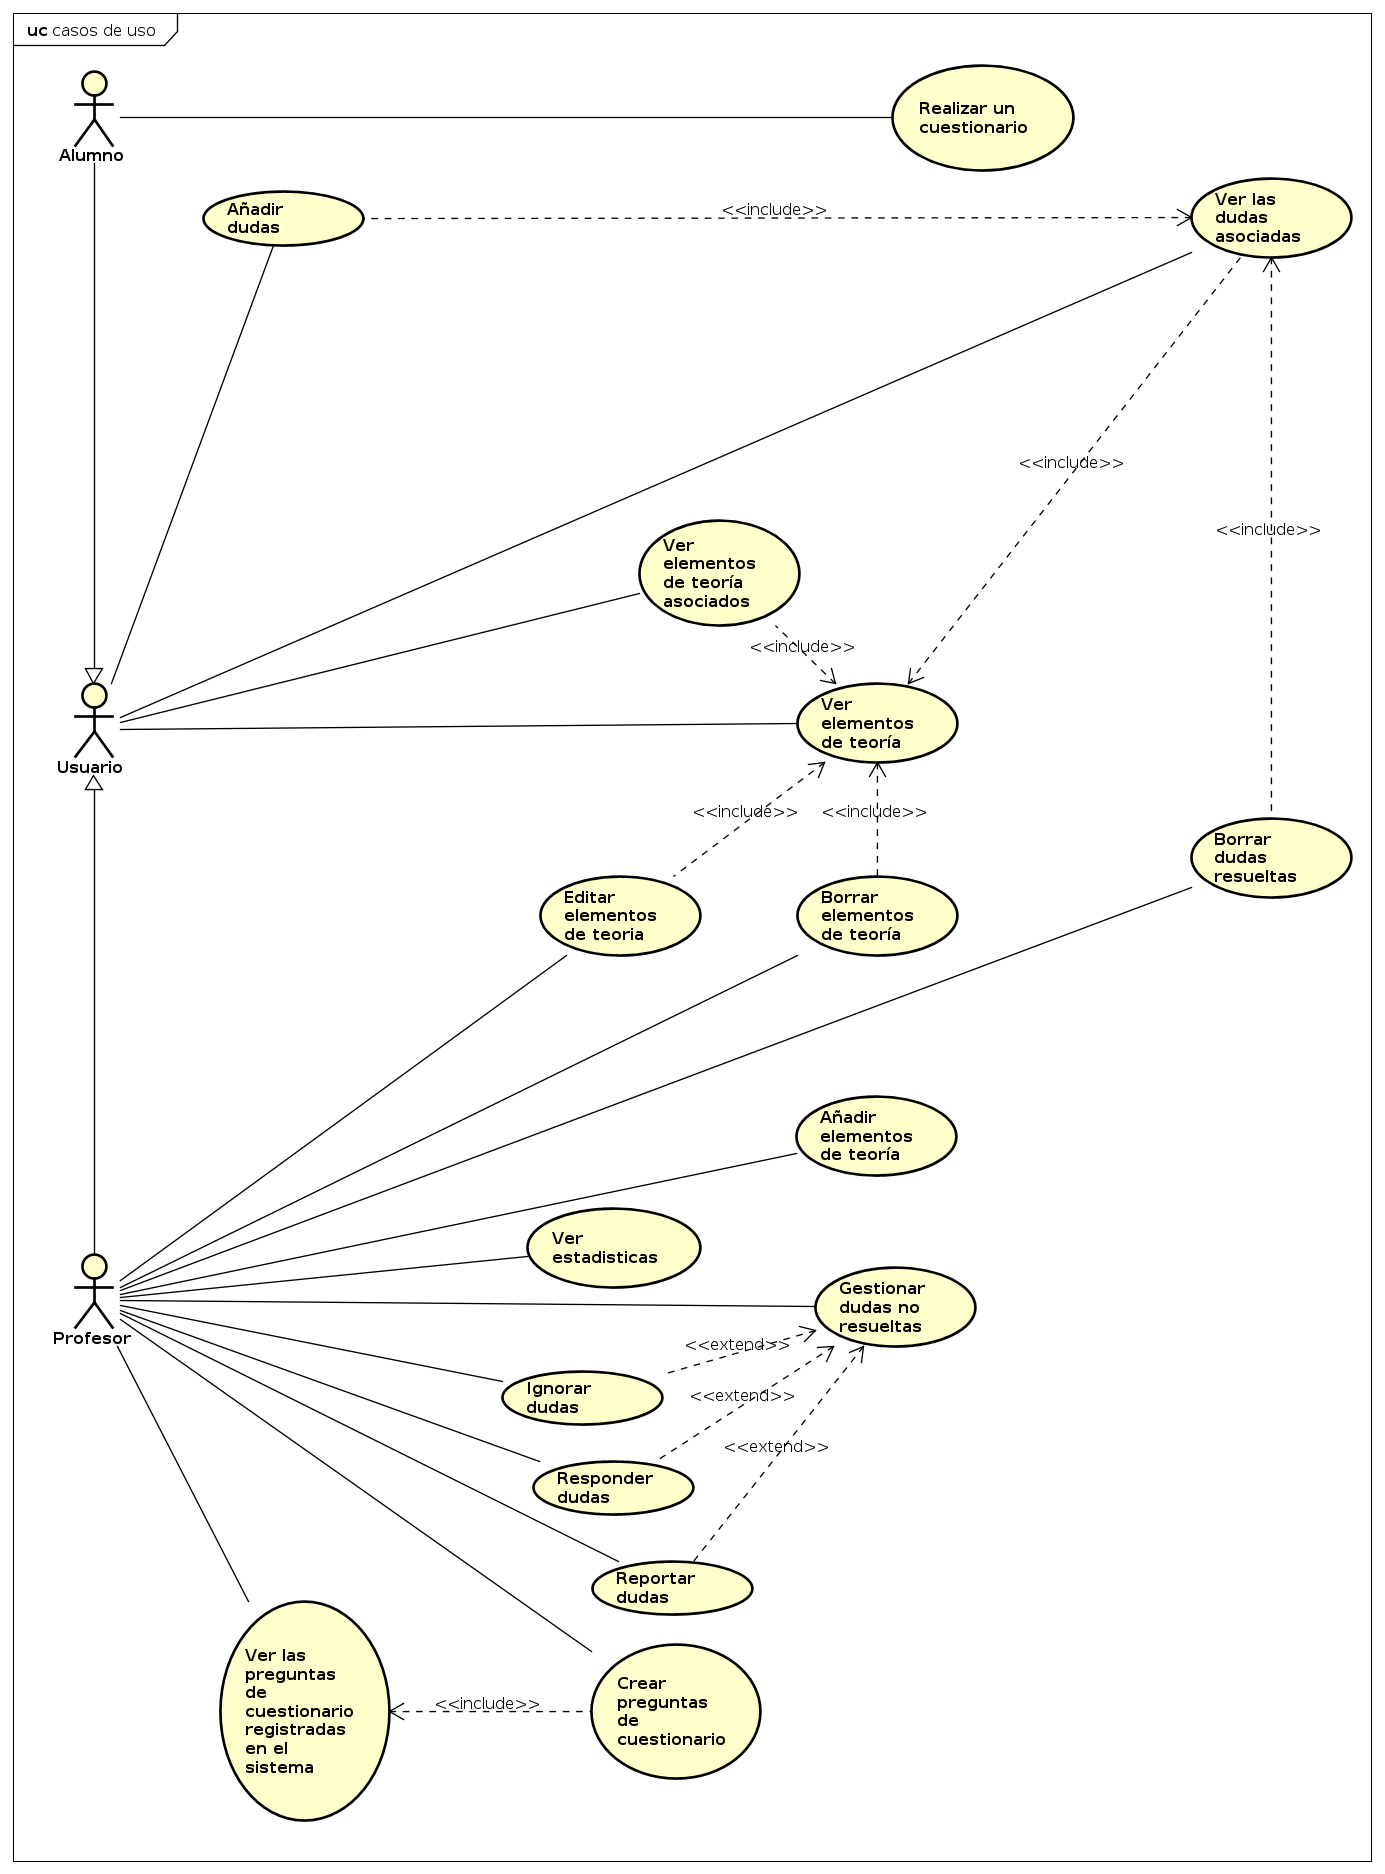
\includegraphics[scale=0.35]{img/astah/analisis/casos_de_uso/useCase00.png}
        \end{center}
        \caption{Diagrama de casos de uso}
    \end{figure}
    
    \newpage
    
    \subsubsection{Descripción de los casos de
    uso}\label{descripciuxf3n-de-los-casos-de-uso}
    
    \vspace*{\fill}
    
    \begin{table}[H]
        \begin{center}
            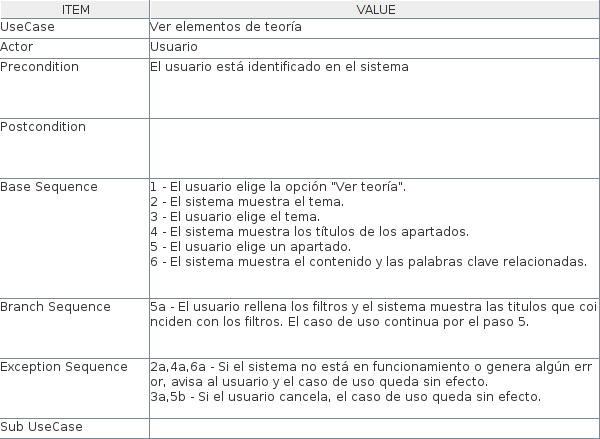
\includegraphics[width=\textwidth]{img/astah/analisis/casos_de_uso/useCase01.png}
        \end{center}
        \caption{Descripción del caso de uso Ver elementos de teoría}
    \end{table}
    
    \vspace*{\fill}
    
    \newpage
    
    \vspace*{\fill}
    
    \begin{table}[H]
        \begin{center}
            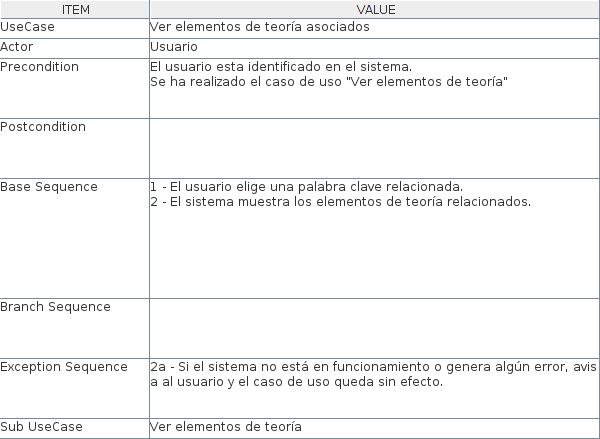
\includegraphics[width=\textwidth]{img/astah/analisis/casos_de_uso/useCase02.png}
        \end{center}
        \caption{Descripción del caso de uso Ver elementos de teoría asociados}
    \end{table}
    
    \vspace*{\fill}
    
    \newpage
    
    \vspace*{\fill}
    
    \begin{table}[H]
        \begin{center}
            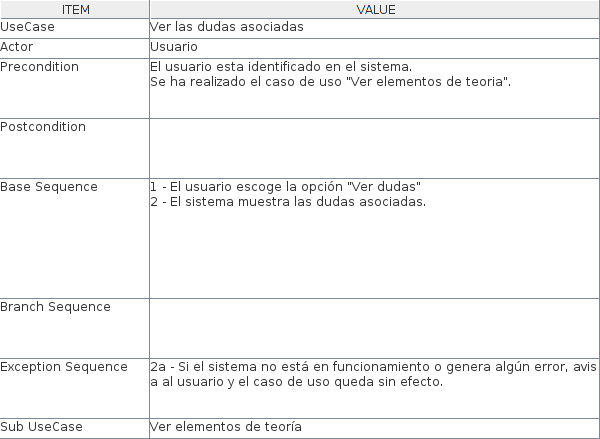
\includegraphics[width=\textwidth]{img/astah/analisis/casos_de_uso/useCase03.png}
        \end{center}
        \caption{Descripción del caso de uso Ver las dudas asociadas}
    \end{table}
    
    \vspace*{\fill}
    
    \newpage
    
    \vspace*{\fill}
    
    \begin{table}[H]
        \begin{center}
            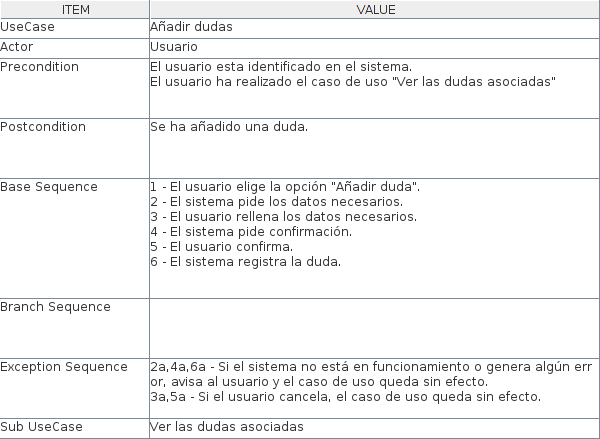
\includegraphics[width=\textwidth]{img/astah/analisis/casos_de_uso/useCase04.png}
        \end{center}
        \caption{Descripción del caso de uso Añadir dudas}
    \end{table}
    
    \vspace*{\fill}
    
    \newpage
    
    \vspace*{\fill}
    
    \begin{table}[H]
        \begin{center}
            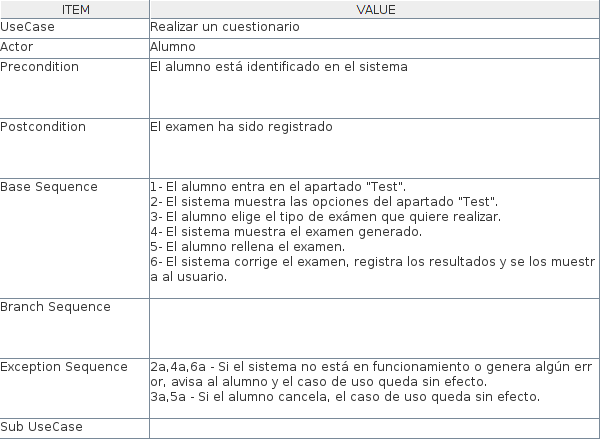
\includegraphics[width=\textwidth]{img/astah/analisis/casos_de_uso/useCase05.png}
        \end{center}
        \caption{Descripción del caso de uso Realizar un cuestionario}
    \end{table}
    
    \vspace*{\fill}
    
    \newpage
    
    \vspace*{\fill}
    
    \begin{table}[H]
        \begin{center}
            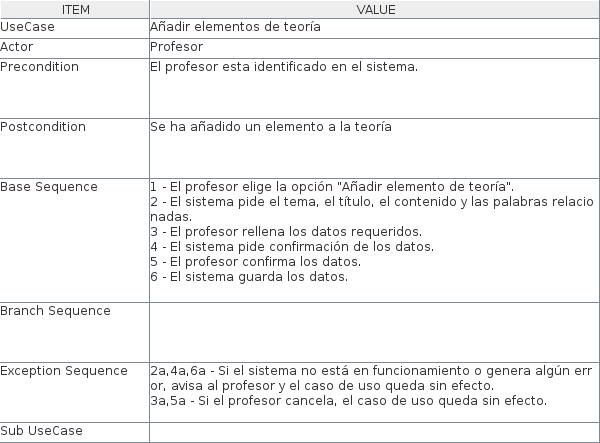
\includegraphics[width=\textwidth]{img/astah/analisis/casos_de_uso/useCase06.png}
        \end{center}
        \caption{Descripción del caso de uso Añadir elementos de teoría}
    \end{table}
    
    \vspace*{\fill}
    
    \newpage
    
    \vspace*{\fill}
    
    \begin{table}[H]
        \begin{center}
            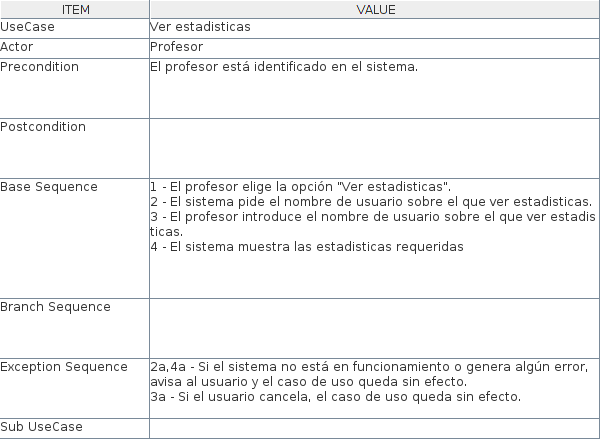
\includegraphics[width=\textwidth]{img/astah/analisis/casos_de_uso/useCase07.png}
        \end{center}
        \caption{Descripción del caso de uso Ver estadísticas}
    \end{table}
    
    \vspace*{\fill}
    
    \newpage
    
    \vspace*{\fill}
    
    \begin{table}[H]
        \begin{center}
            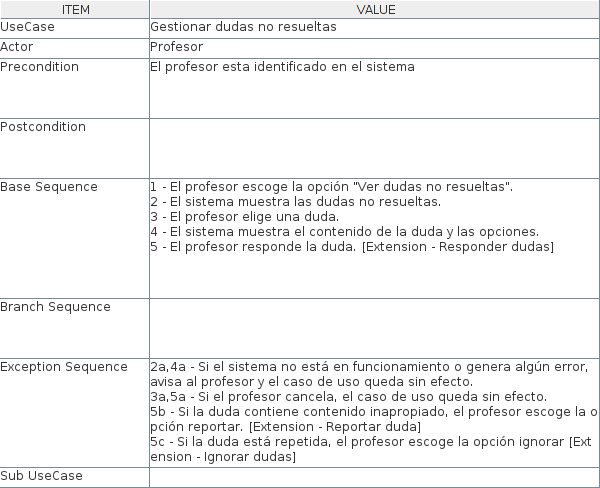
\includegraphics[width=\textwidth]{img/astah/analisis/casos_de_uso/useCase08.png}
        \end{center}
        \caption{Descripción del caso de uso Gestionar dudas no resueltas}
    \end{table}
    
    \vspace*{\fill}
    
    \newpage
    
    \vspace*{\fill}
    
    \begin{table}[H]
        \begin{center}
            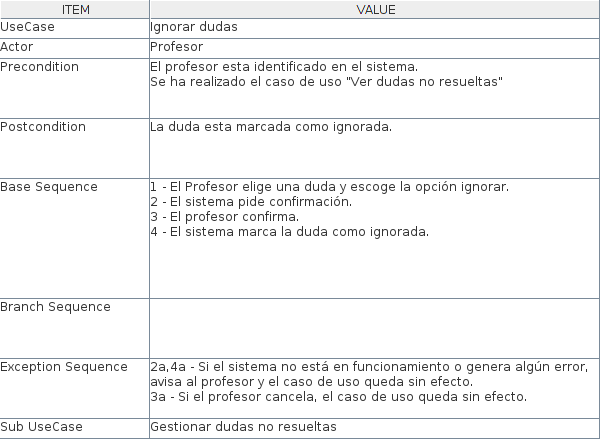
\includegraphics[width=\textwidth]{img/astah/analisis/casos_de_uso/useCase09.png}
        \end{center}
        \caption{Descripción del caso de uso Ignorar dudas}
    \end{table}
    
    \vspace*{\fill}
    
    \newpage
    
    \vspace*{\fill}
    
    \begin{table}[H]
        \begin{center}
            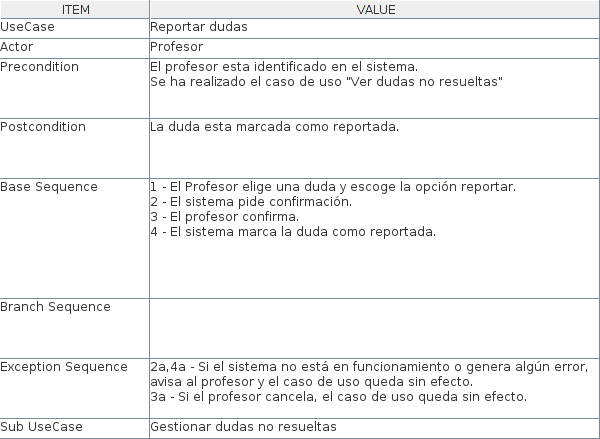
\includegraphics[width=\textwidth]{img/astah/analisis/casos_de_uso/useCase10.png}
        \end{center}
        \caption{Descripción del caso de uso Reportar dudas}
    \end{table}
    
    \vspace*{\fill}
    
    \newpage
    
    \vspace*{\fill}
    
    \begin{table}[H]
        \begin{center}
            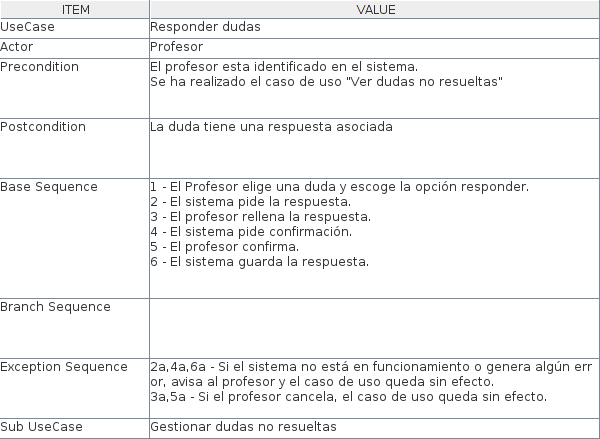
\includegraphics[width=\textwidth]{img/astah/analisis/casos_de_uso/useCase11.png}
        \end{center}
        \caption{Descripción del caso de uso Responder dudas}
    \end{table}
    
    \vspace*{\fill}
    
    \newpage
    
    \vspace*{\fill}
    
    \begin{table}[H]
        \begin{center}
            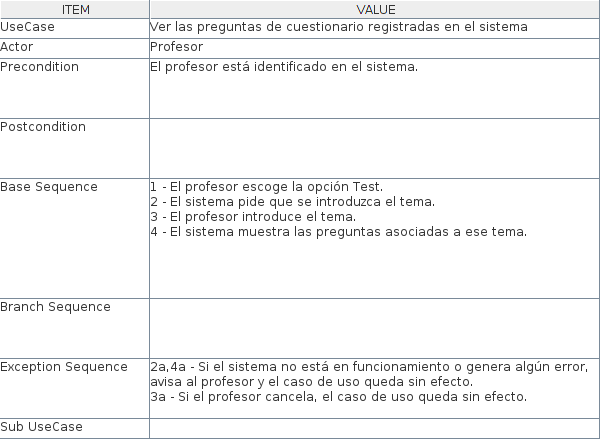
\includegraphics[width=\textwidth]{img/astah/analisis/casos_de_uso/useCase12.png}
        \end{center}
        \caption{Descripción del caso de uso Ver las preguntas de cuestionario registradas en el sistema}
    \end{table}
    
    \vspace*{\fill}
    
    \newpage
    
    \vspace*{\fill}
    
    \begin{table}[H]
        \begin{center}
            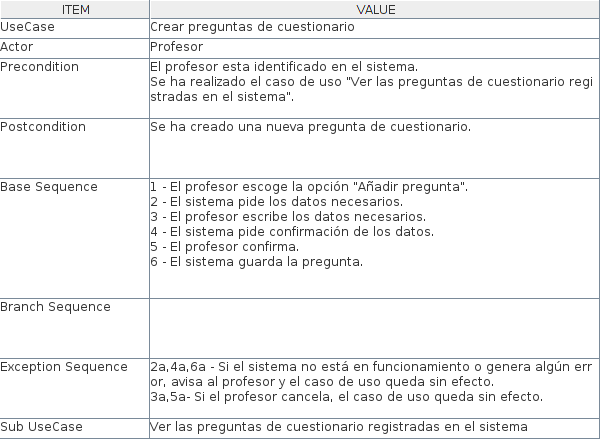
\includegraphics[width=\textwidth]{img/astah/analisis/casos_de_uso/useCase13.png}
        \end{center}
        \caption{Descripción del caso de uso Crear preguntas de cuestionario}
    \end{table}
    
    \vspace*{\fill}
    
    \newpage
    
    \vspace*{\fill}
    
    \begin{table}[H]
        \begin{center}
            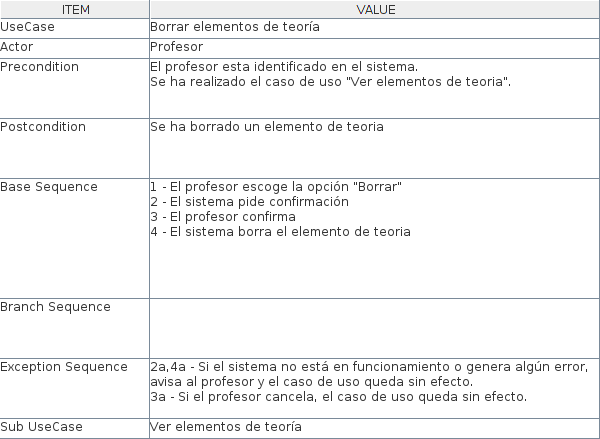
\includegraphics[width=\textwidth]{img/astah/analisis/casos_de_uso/useCase14.png}
        \end{center}
        \caption{Descripción del caso de uso Borrar elementos de teoría}
    \end{table}
    
    \vspace*{\fill}
    
    \newpage
    
    \vspace*{\fill}
    
    \begin{table}[H]
        \begin{center}
            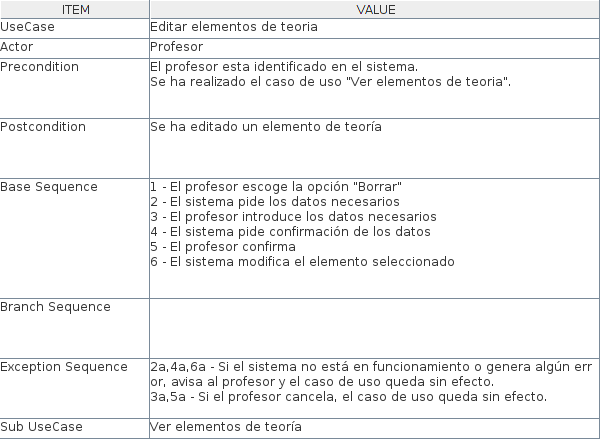
\includegraphics[width=\textwidth]{img/astah/analisis/casos_de_uso/useCase15.png}
        \end{center}
        \caption{Descripción del caso de uso Editar elementos de teoria}
    \end{table}
    
    \vspace*{\fill}
    
    \newpage
    
    \vspace*{\fill}
    
    \begin{table}[H]
        \begin{center}
            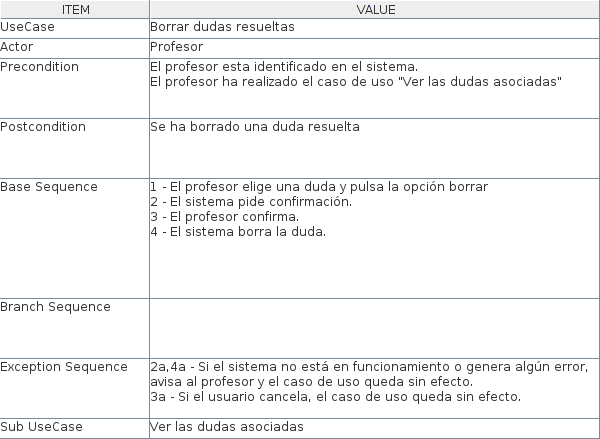
\includegraphics[width=\textwidth]{img/astah/analisis/casos_de_uso/useCase16.png}
        \end{center}
        \caption{Descripción del caso de uso Borrar dudas resueltas}
    \end{table}
    
    \vspace*{\fill} \newpage
    
    \subsection{Modelo de dominio}\label{modelo-de-dominio}
    
    \vspace*{\fill}
    
    \begin{figure}[H]
        \begin{center}
            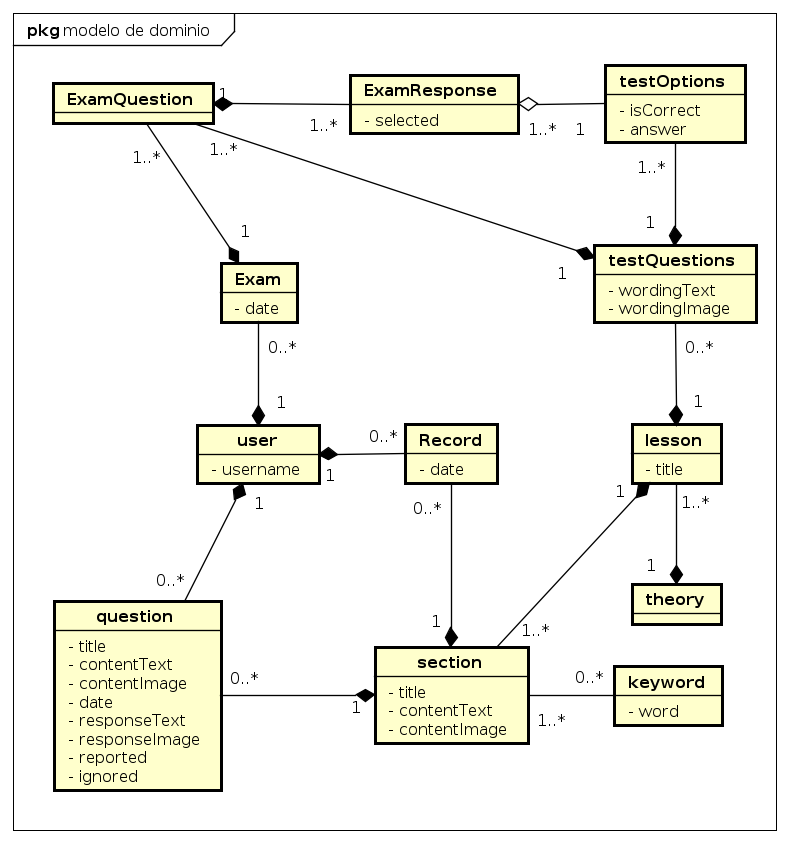
\includegraphics[width=\textwidth]{img/astah/analisis/dominio/modelo.png}
        \end{center}
        \caption{Modelo de dominio}
    \end{figure}
    
    \vspace*{\fill}
    
    \section{Diseño}\label{diseuxf1o}
    
    \subsection{Diseño de la base de
    datos}\label{diseuxf1o-de-la-base-de-datos}
    
    \vspace*{\fill}
    
    \begin{figure}[H]
        \begin{center}
            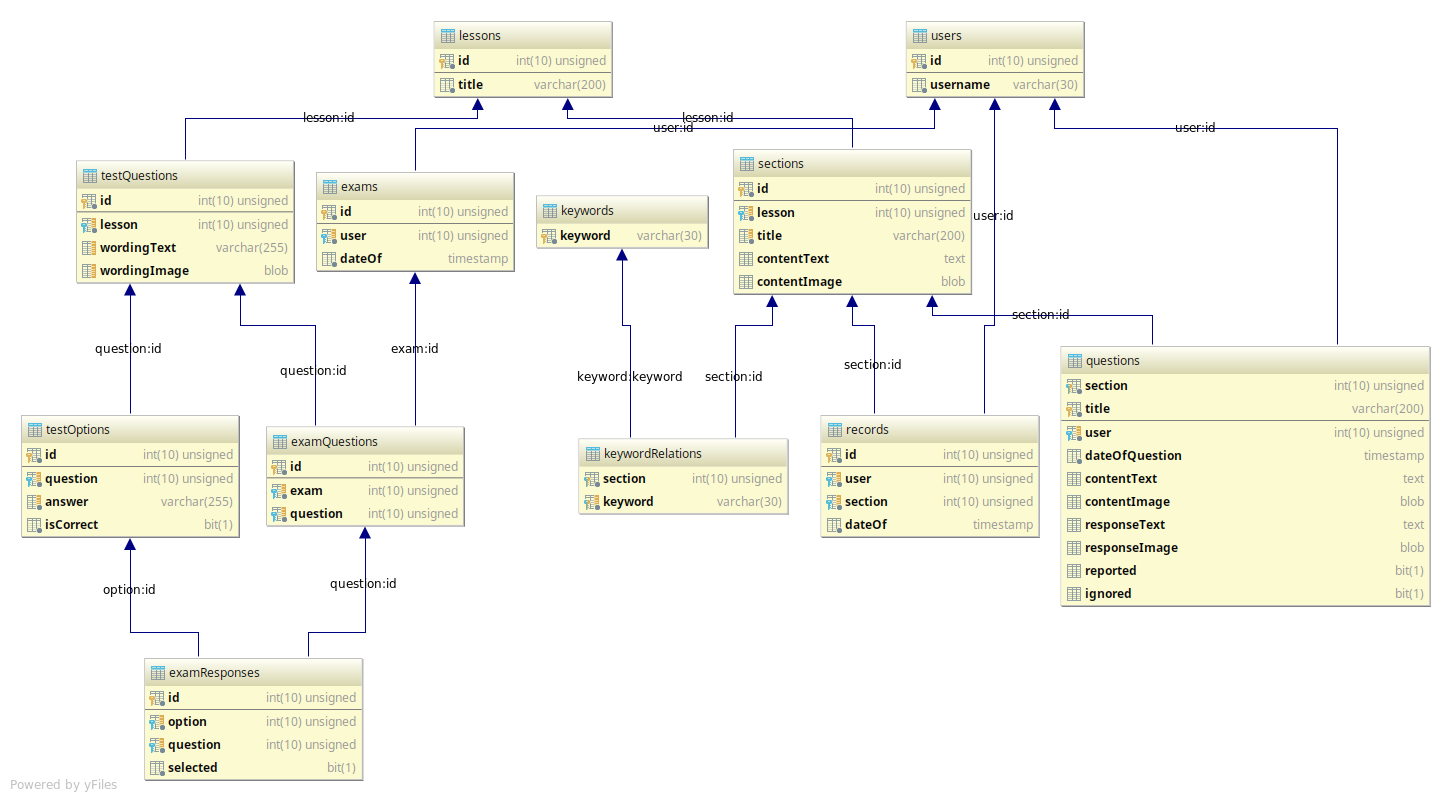
\includegraphics[width=\textwidth, angle=-90]{img/astah/disenio/relacional/diagram.png}
        \end{center}
        \caption{Diagrama relacional}
    \end{figure}
    
    \vspace*{\fill} \newpage
    
    \subsection{Despliegue}\label{despliegue}
    
    \vspace*{\fill}
    
    \begin{figure}[H]
        \begin{center}
            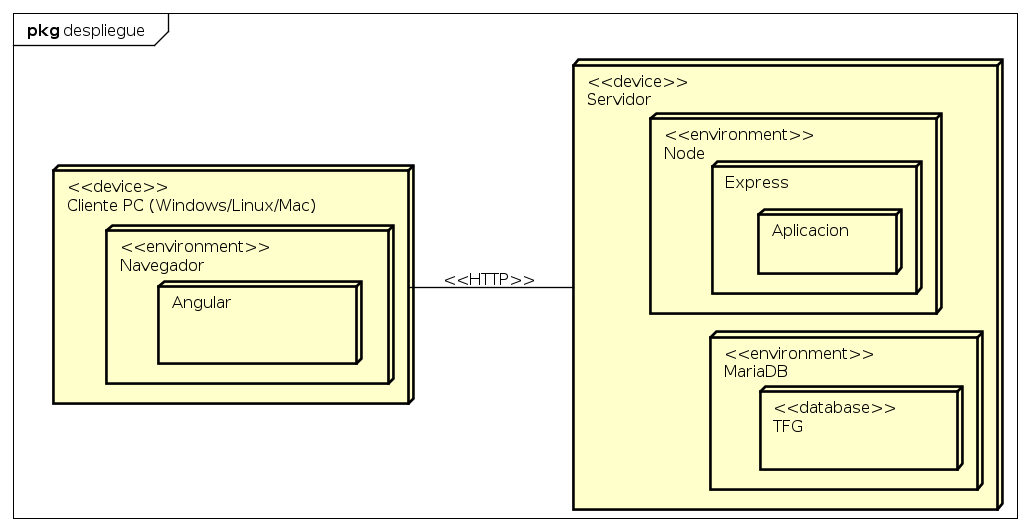
\includegraphics[width=\textwidth, angle=-90]{img/astah/disenio/despliegue/deployment.png}
        \end{center}
        \caption{Diagrama de despliegue}
    \end{figure}
    
    \vspace*{\fill} \newpage
    
    \subsection{Descomposición modular}\label{descomposiciuxf3n-modular}
    
    \subsubsection{Front-end}\label{front-end}
    
    \vspace*{\fill}
    
    \begin{figure}[H]
        \begin{center}
            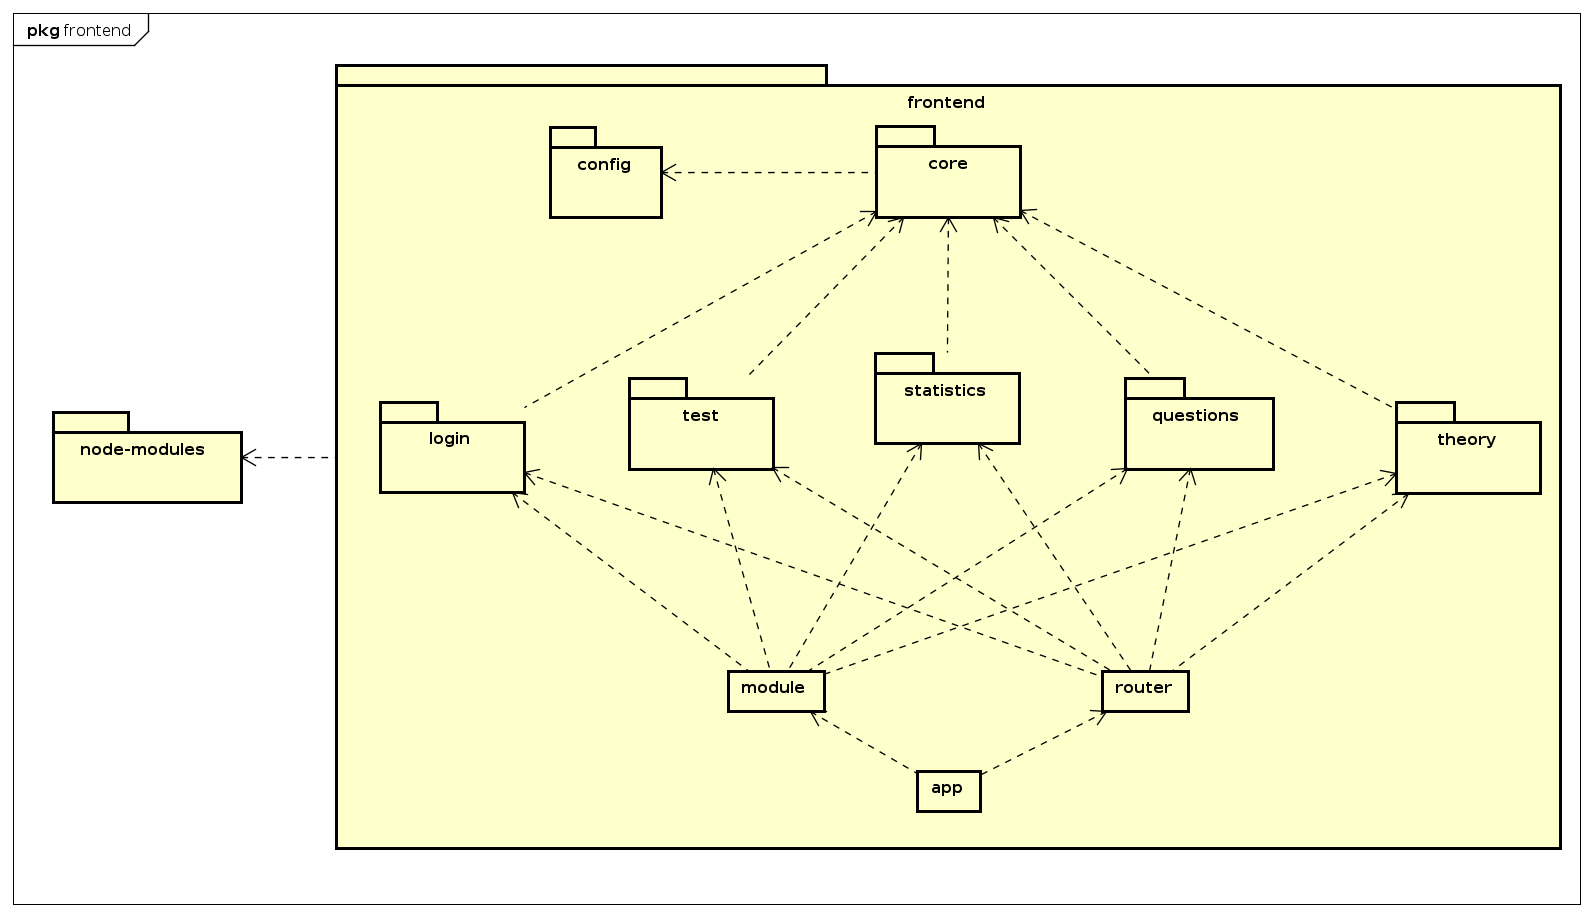
\includegraphics[width=\textwidth, angle=-90]{img/astah/disenio/descomposicion/front/descomposicion.png}
        \end{center}
        \caption{Diagrama de descomposición modular frontend}
    \end{figure}
    
    \vspace*{\fill} \newpage
    
    \vspace*{\fill}
    
    \begin{figure}[H]
        \begin{center}
            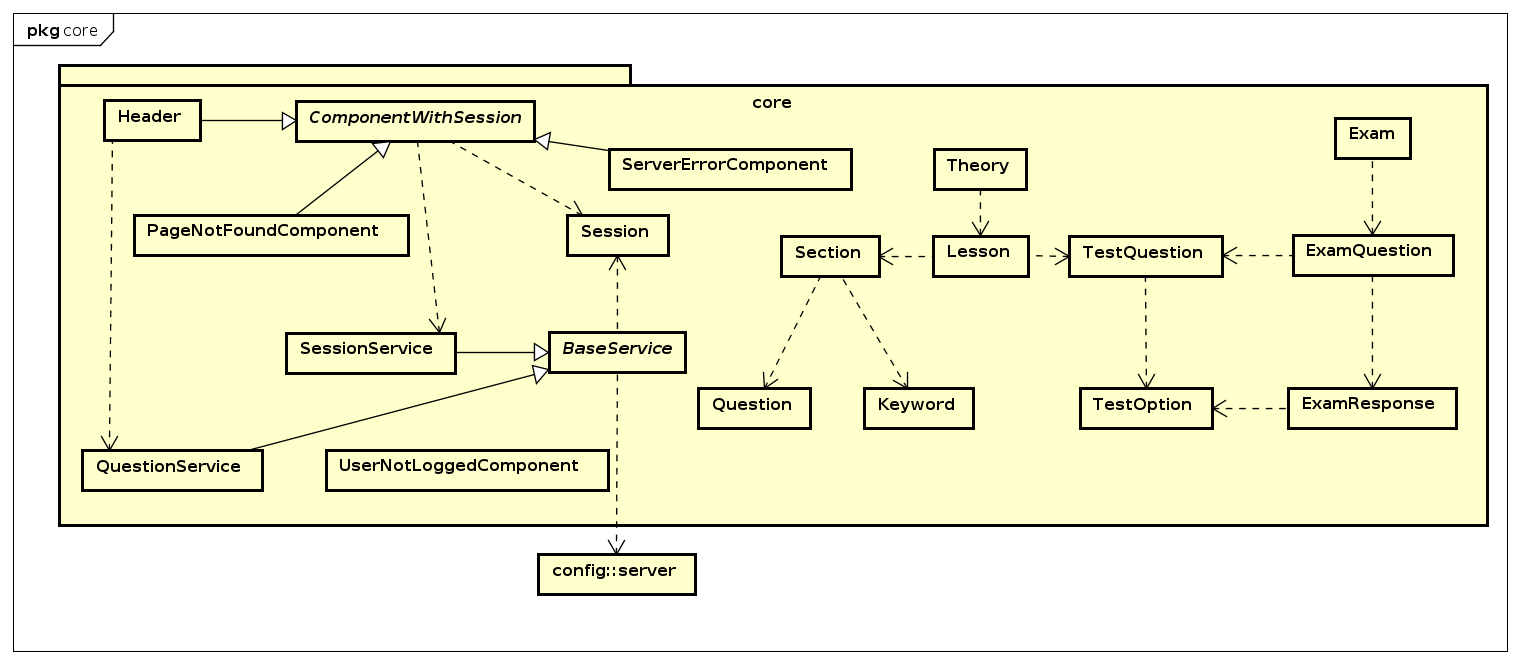
\includegraphics[width=\textwidth, angle=-90]{img/astah/disenio/descomposicion/front/core.png}
        \end{center}
        \caption{Diagrama de descomposición modular frontend-core}
    \end{figure}
    
    \vspace*{\fill} \newpage
    
    \vspace*{\fill}
    
    \begin{figure}[H]
        \begin{center}
            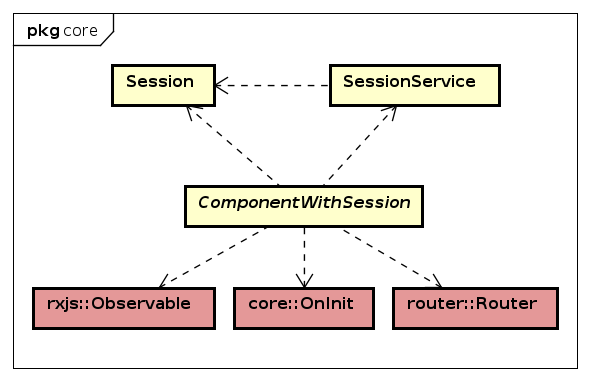
\includegraphics[width=\textwidth, angle=-90]{img/astah/disenio/descomposicion/front/ejemploComponente.png}
        \end{center}
        \caption{Diagrama de ejemplo de un componente}
    \end{figure}
    
    \vspace*{\fill} \newpage
    
    \vspace*{\fill}
    
    \begin{figure}[H]
        \begin{center}
            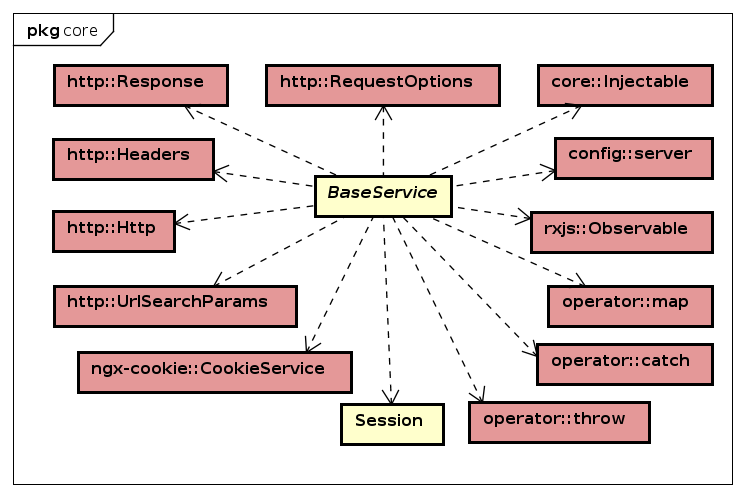
\includegraphics[width=\textwidth, angle=-90]{img/astah/disenio/descomposicion/front/ejemploServicio.png}
        \end{center}
        \caption{Diagrama de ejemplo de un servicio}
    \end{figure}
    
    \vspace*{\fill} \newpage
    
    \vspace*{\fill}
    
    \begin{figure}[H]
        \begin{center}
            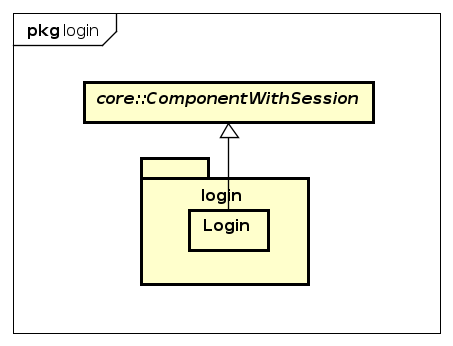
\includegraphics[width=\textwidth]{img/astah/disenio/descomposicion/front/login.png}
        \end{center}
        \caption{Diagrama de descomposición modular frontend-login}
    \end{figure}
    
    \vspace*{\fill} \newpage
    
    \vspace*{\fill}
    
    \begin{figure}[H]
        \begin{center}
            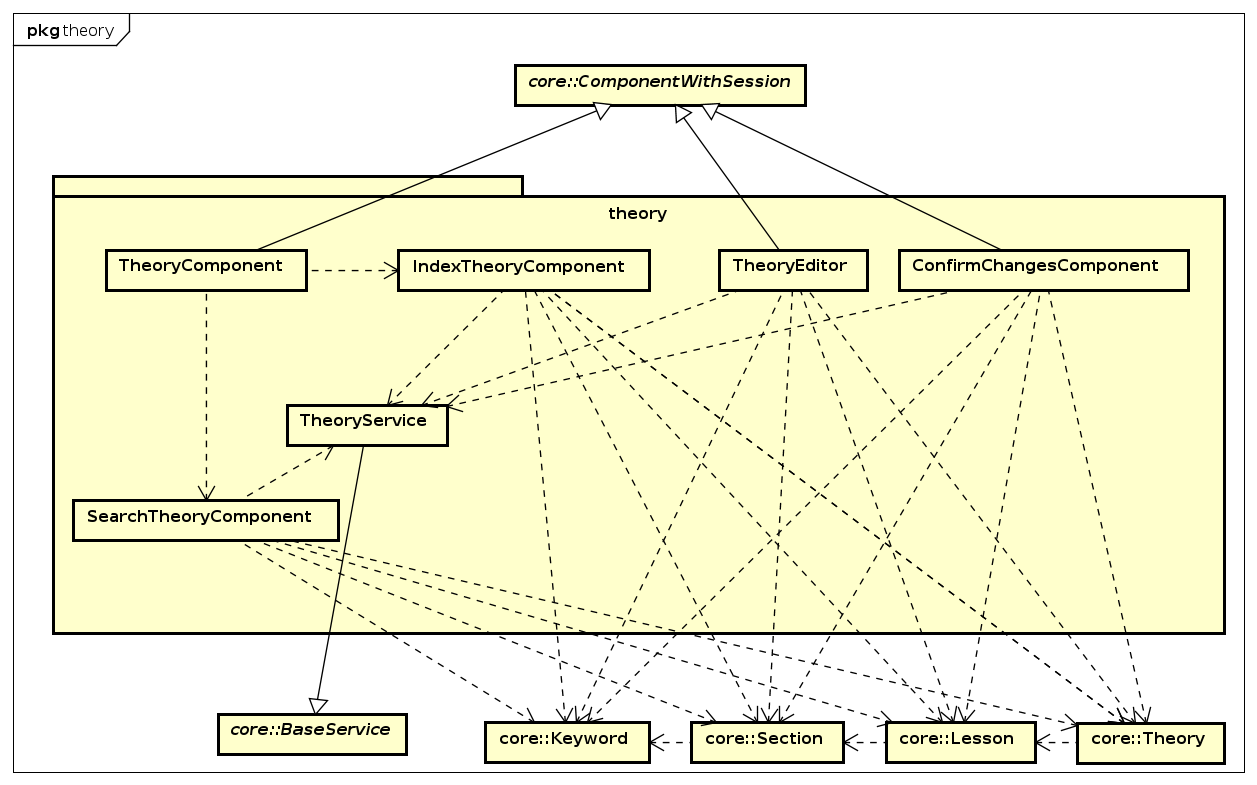
\includegraphics[width=\textwidth, angle=-90]{img/astah/disenio/descomposicion/front/theory.png}
        \end{center}
        \caption{Diagrama de descomposición modular frontend-theory}
    \end{figure}
    
    \vspace*{\fill} \newpage
    
    \vspace*{\fill}
    
    \begin{figure}[H]
        \begin{center}
            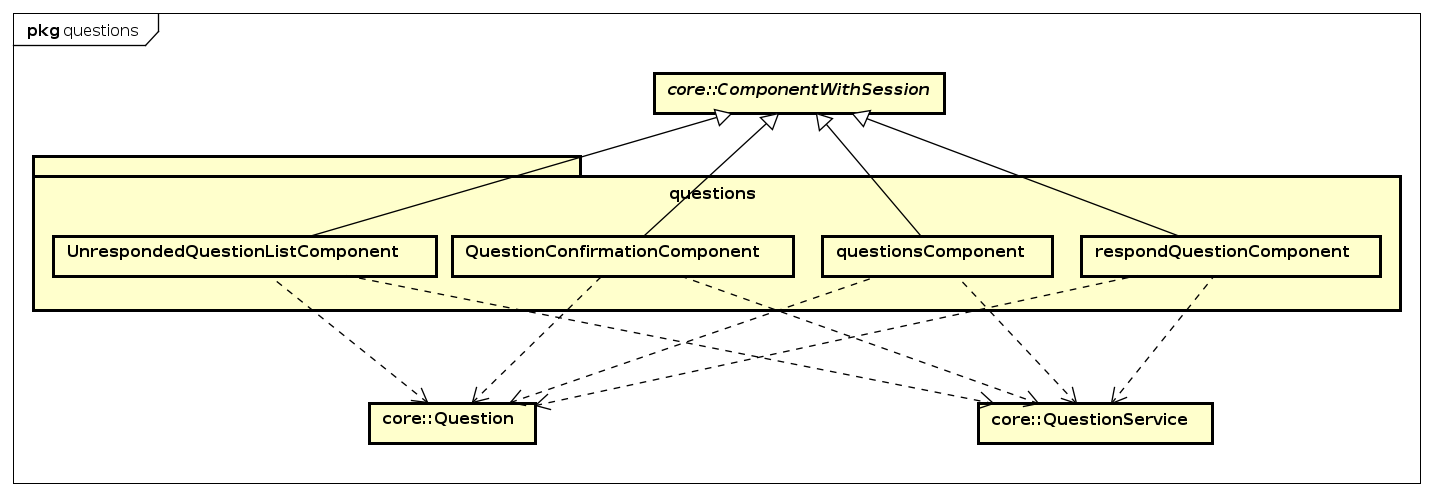
\includegraphics[width=\textwidth, angle=-90]{img/astah/disenio/descomposicion/front/questions.png}
        \end{center}
        \caption{Diagrama de descomposición modular frontend-questions}
    \end{figure}
    
    \vspace*{\fill} \newpage
    
    \vspace*{\fill}
    
    \begin{figure}[H]
        \begin{center}
            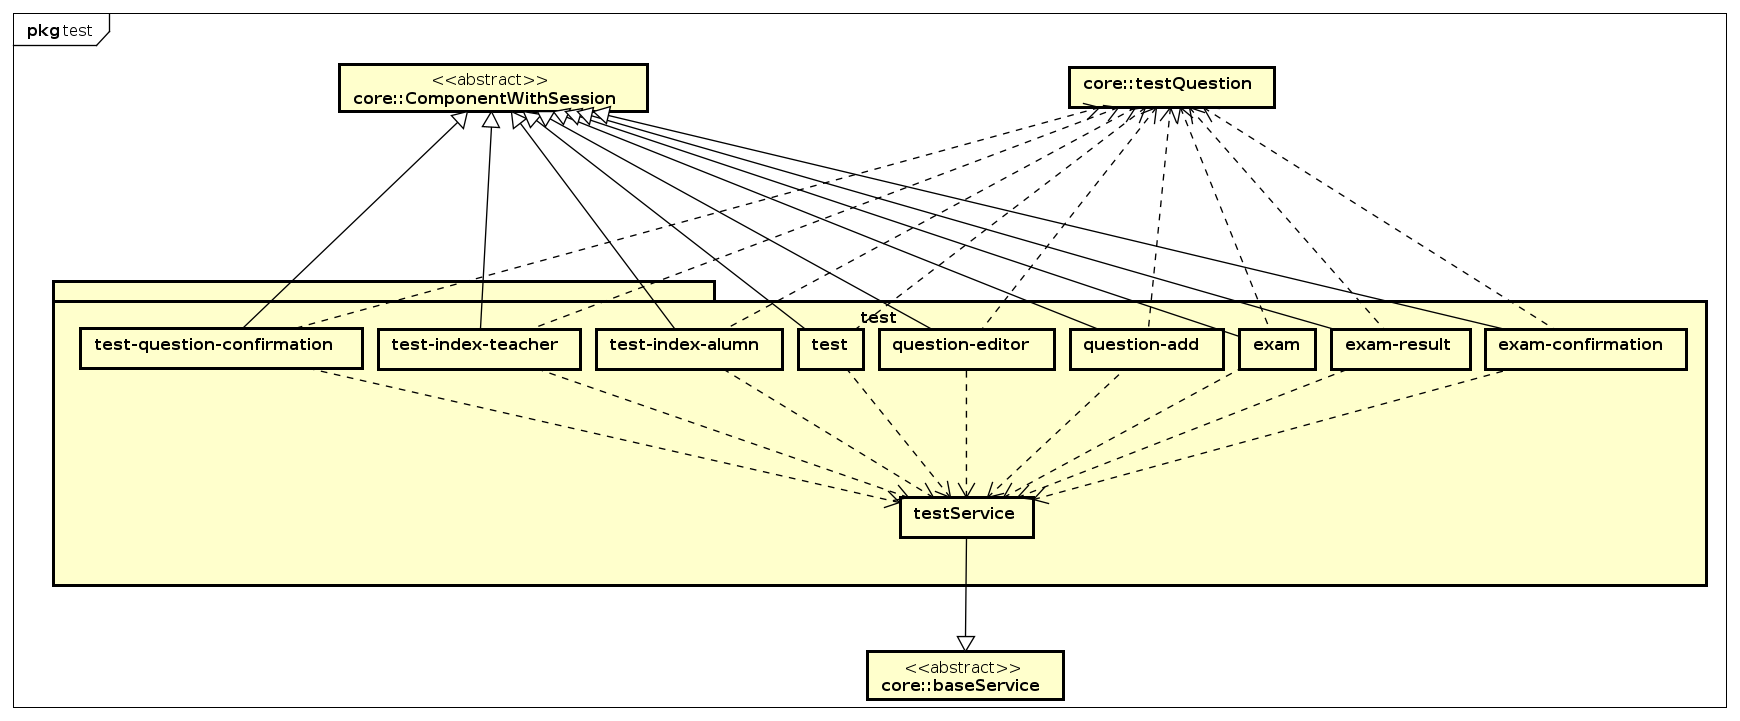
\includegraphics[width=\textwidth, angle=-90]{img/astah/disenio/descomposicion/front/test.png}
        \end{center}
        \caption{Diagrama de descomposición modular frontend-test}
    \end{figure}
    
    \vspace*{\fill} \newpage
    
    \vspace*{\fill}
    
    \begin{figure}[H]
        \begin{center}
            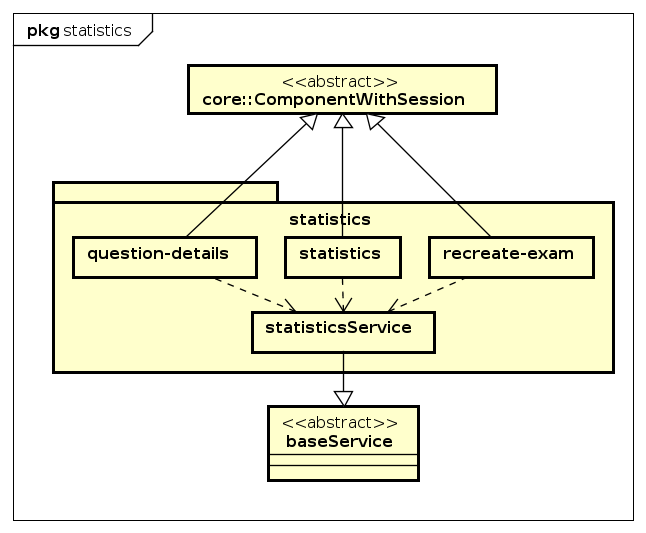
\includegraphics[width=\textwidth, angle=-90]{img/astah/disenio/descomposicion/front/statistics.png}
        \end{center}
        \caption{Diagrama de descomposición modular frontend-statistics}
    \end{figure}
    
    \vspace*{\fill} \newpage
    
    \subsubsection{Back-end}\label{back-end}
    
    \vspace*{\fill}
    
    \begin{figure}[H]
        \begin{center}
            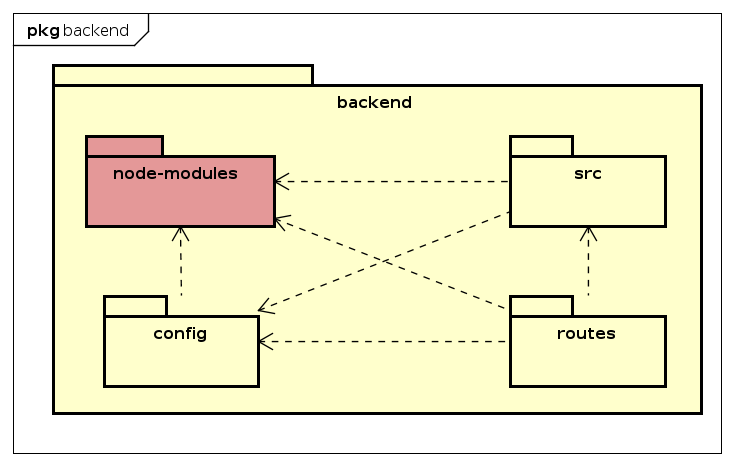
\includegraphics[width=\textwidth]{img/astah/disenio/descomposicion/back/back.png}
        \end{center}
        \caption{Diagrama de descomposición modular backend}
    \end{figure}
    
    \vspace*{\fill} \newpage
    \vspace*{\fill}
    
    \begin{figure}[H]
        \begin{center}
            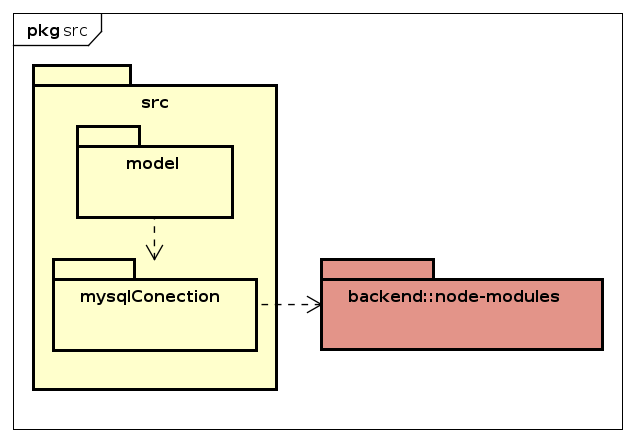
\includegraphics[width=\textwidth]{img/astah/disenio/descomposicion/back/src.png}
        \end{center}
        \caption{Diagrama de descomposición modular backend-src}
    \end{figure}
    
    \vspace*{\fill} \newpage
    \vspace*{\fill}
    
    \begin{figure}[H]
        \begin{center}
            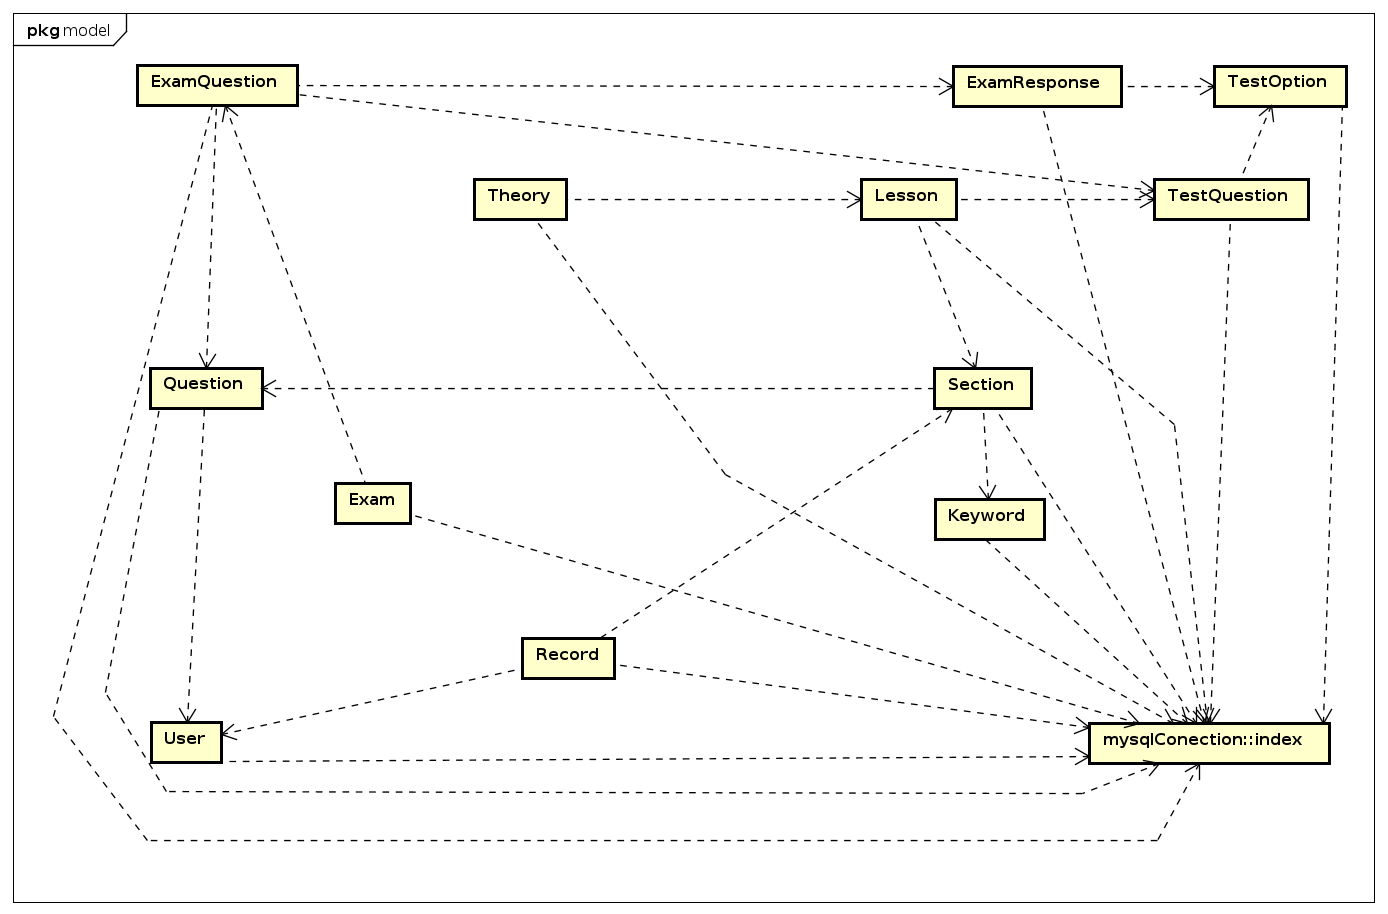
\includegraphics[width=\textwidth, angle=-90]{img/astah/disenio/descomposicion/back/model.png}
        \end{center}
        \caption{Diagrama de descomposición modular backend-model}
    \end{figure}
    
    \vspace*{\fill} \newpage
    
    \subsection{Diagrama de clases}\label{diagrama-de-clases}
    
    \vspace*{\fill}
    
    \begin{figure}[H]
        \begin{center}
            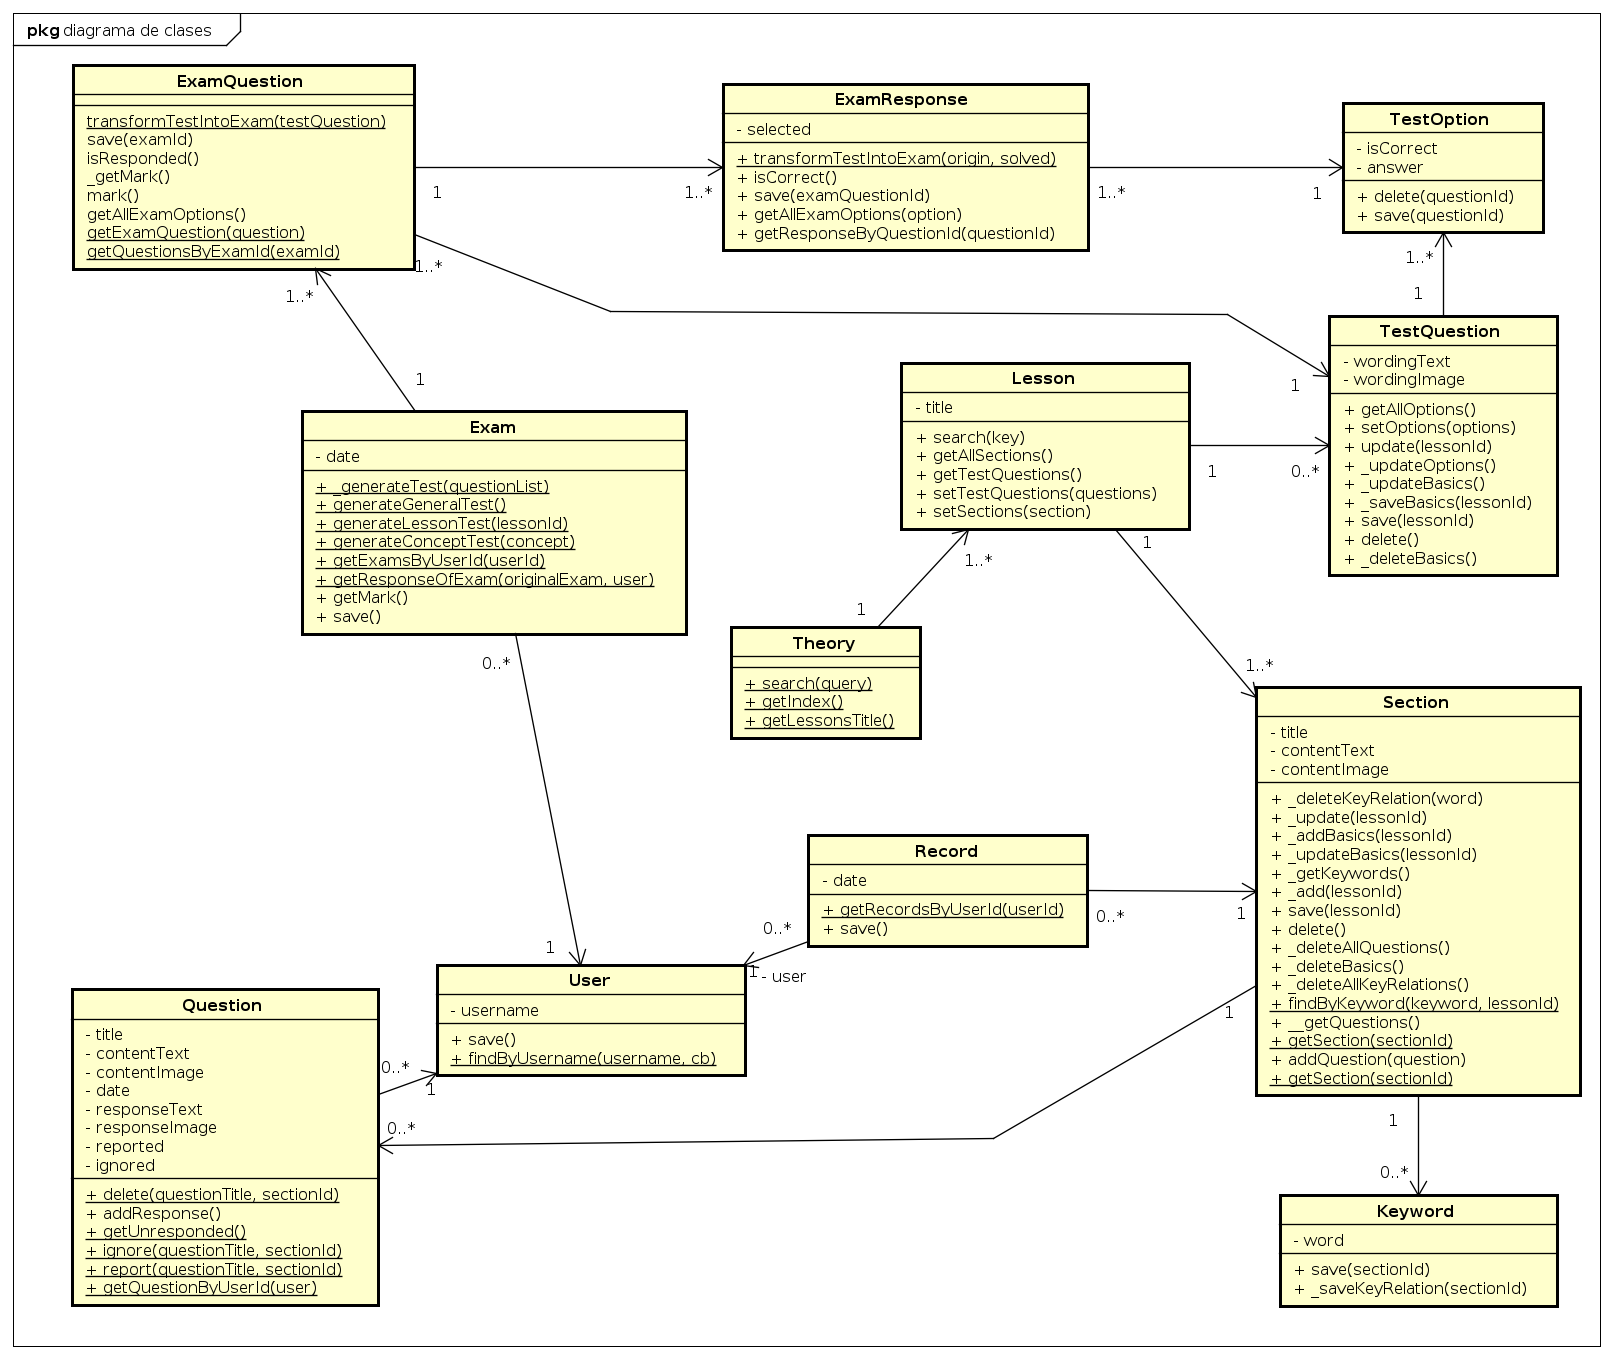
\includegraphics[width=\textwidth, angle=-90]{img/astah/disenio/clases/clasesNavegable.png}
        \end{center}
        \caption{Diagrama de clases}
    \end{figure}
    
    \vspace*{\fill} \newpage
    
    \vspace*{\fill}
    
    \begin{figure}[H]
        \begin{center}
            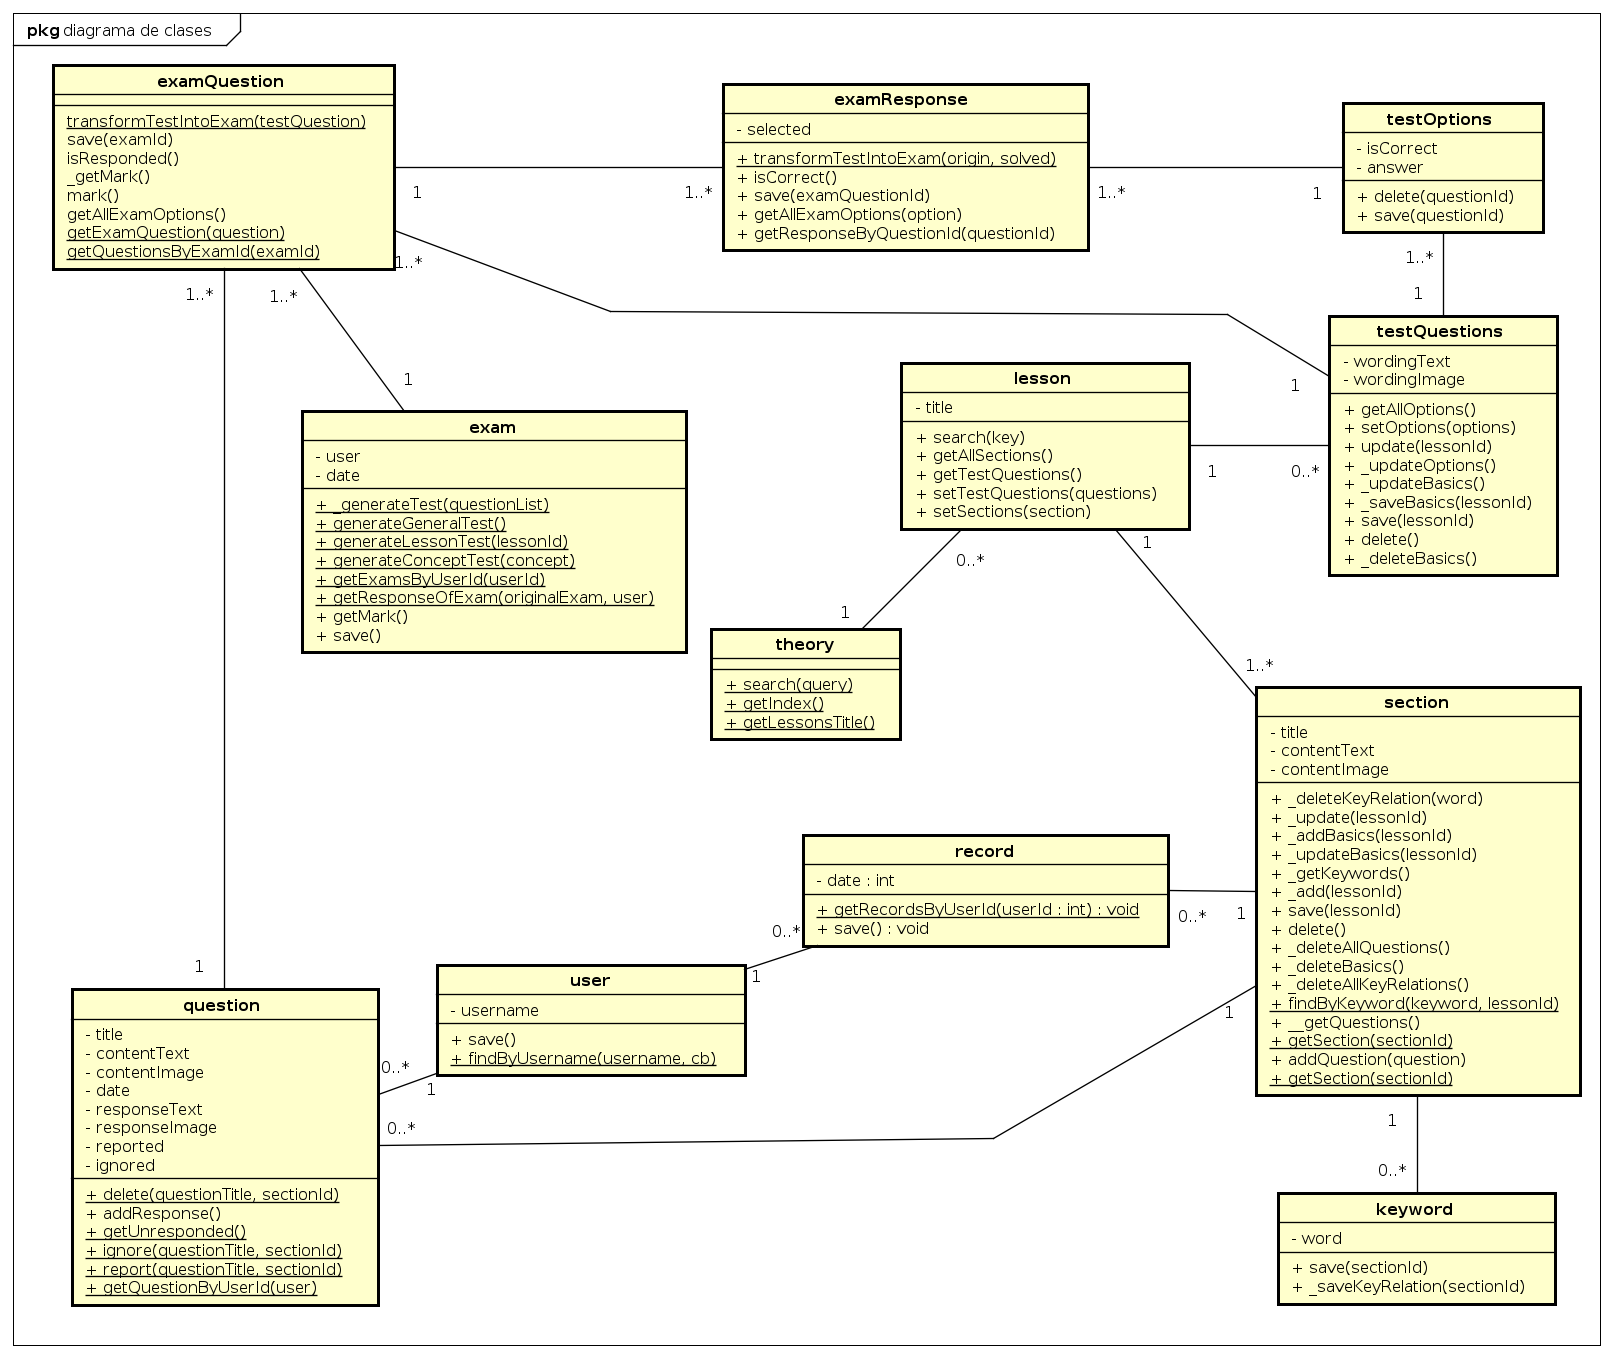
\includegraphics[width=\textwidth, angle=-90]{img/astah/disenio/clases/clases.png}
        \end{center}
        \caption{Diagrama de clases}
    \end{figure}
    
    \vspace*{\fill} \newpage
    
    \chapter{ Conclusiones }
    
    Se han cumplido la mayoría de objetivos iniciales, desarrollando todas
    las funcionalidades previstas salvo las relacionadas con la herramienta
    práctica. Tal y como se explica en el capítulo 3, debido a una mala
    planificación inicial, se descartó realizar las funcionalidades
    relacionadas con una herramienta práctica que permitiría al alumno poner
    en práctica los conocimientos teóricos estudiados.
    
    Se ha desarrollado una interfaz sencilla y clara, orientada a
    ordenadores de sobremesa.
    
    Durante la realización del proyecto se han adquirido y mejorado nuevos
    conocimientos del desarrollo web y lenguajes de programación. Se ha
    aprendido en profundidad el funcionamiento de Angular, Node, Bootstrap 4
    y Express.
    
    \section{Trabajo futuro}\label{trabajo-futuro}
    
    En el futuro se le podría añadir mayor funcionalidad a la aplicación,
    aumentando su potencial. Algunas de las que han ido surgiendo durante la
    relación de este trabajo son:
    
    \begin{itemize}
    \tightlist
    \item
      Mejora de la interfaz, para hacerla más atractiva para el usuario
    \item
      Adecuar el diseño a los dispositivos móviles.
    \item
      Añadir la funcionalidad \enquote{herramienta práctica} que fue
      eliminada durante el desarrollo del proyecto.
    \item
      Añadir nuevas funcionalidades, como la de permitir al profesor
      pregenerar un cuestionario específico con un número determinado de
      preguntas generadas aleatoriamente o bien seleccionadas por el
      profesor de entre las introducidas previamente en la aplicación. Estos
      cuestionarios prodían ser utilizados para las pruebas de evaluación
      contínua.
    \item
      Aumentar las estadísticas recogidas, así como generar gráficas que
      muestren los datos.
    \end{itemize}
    
    \appendix
    
    \chapter{ Manual de despliegue }
    
    Para desplegar esta aplicación necesitamos:
    
    \begin{itemize}
    \item
      Un ordenador con un sistema operativo basado en UNIX con node y npm
      instalados
    \item
      Conexión a Internet(para descargar dependencias)
    \item
      El código fuente de la aplicación.
    
      Aunque se entrega en el CD, esta disponible en
      https://github.com/Raikuro/TFG
    \end{itemize}
    
    Pasos a realizar para desplegar:
    
    \begin{enumerate}
    \def\labelenumi{\arabic{enumi}.}
    \tightlist
    \item
      \textbf{Modificar los ficheros de configuración:}
    \end{enumerate}
    
    Para entenderlos ficheros de configuración se explica la máquina en la
    que está actualmente desplegada la aplicación.
    
    La máquina es accesible mediante la dirección
    \enquote{http://virtual.lab.inf.uva.es} en el puerto 20052. Debido a la
    configuración interna de la máquina, redirige el puerto interno 80 al
    puerto externo 20052 y el puerto 3000 al 20053.
    
    Los ficheros que es necesario modificar son los siguientes:
    
    \begin{itemize}
    \item
      backend/config/client.js:
    
    \begin{verbatim}
    const IP = 'http://virtual.lab.inf.uva.es'
    const PORT = 20052 
    exports.ADDRESS = IP + ':' + PORT
    \end{verbatim}
    
      Es necesario cambiar las constantes IP y PORT por la IP y el puerto
      desde el cual será accesible nuestro frontend.
    \item
      frontend/.angular-cli.json:
    
    \begin{verbatim}
    ...
    "defaults": {
      "styleExt": "css",
    "component": {},
    "serve": {
      "host": "10.0.20.5",
      "port": 80
    }
      }
    ...
    \end{verbatim}
    
      Es necesario cambiar los parámetros host y port por la IP y el puerto
      interno en el que desplegaremos nuestro frontend
    \item
      frontend/src/app/config/server.ts
    
    \begin{verbatim}
    const IP = "http://virtual.lab.inf.uva.es";
    const PORT = 20053;
    export const ADDRESS = IP + ":" + PORT
    \end{verbatim}
    
      Es necesario cambiar las constantes IP y PORT por la IP y el puerto
      desde el cual será accesible nuestro backend
    \end{itemize}
    
    \begin{enumerate}
    \def\labelenumi{\arabic{enumi}.}
    \setcounter{enumi}{1}
    \tightlist
    \item
      \textbf{Instalar las dependencias:}
    \end{enumerate}
    
    Se ejecutarán los siguientes comandos desde la raiz del CD
    
    \begin{verbatim}
    cd backend
    npm install
    cd frontend
    npm install
    \end{verbatim}
    
    \begin{enumerate}
    \def\labelenumi{\arabic{enumi}.}
    \setcounter{enumi}{2}
    \tightlist
    \item
      \textbf{Desplegar:}
    \end{enumerate}
    
    Se ejecutarán los siguientes comandos desde la raiz del CD para
    desplegar el frontend
    
    \begin{verbatim}
    cd frontend
    npm start
    \end{verbatim}
    
    Se ejecutarán los siguientes comandos desde la raiz del CD para
    desplegar el backend
    
    \begin{verbatim}
    cd backend
    npm start
    \end{verbatim}
    
    \chapter{ Manual de usuario }
    
    A continuación, se explicará el funcionamiento de la aplicación web.
    
    Como primer pantalla, está la página de inicio de sesión. El usuario
    debe introducir su nombre de usuario de la universidad y su contraseña.
    
    \begin{figure}[H]
        \begin{center}
            
\includegraphics[width=\textwidth]{img/manual/login.png}
        \end{center}
        \caption{Pantalla de inicio de sesión}
    \end{figure}
    
    Distinguiremos dos casos, según sea un alumno o un profesor el que
    ingrese en la aplicación.
    
    \newpage
    
    \section{Manual del alumno:}\label{manual-del-alumno}
    
    Según se ingresa en la aplicación se accede a la pantalla de teoría. Se
    puede ver en la parte superior la barra de navegación, y en ella dos
    apartados, \enquote{Teoría} y \enquote{Test} y la opción
    \enquote{Salir}. Esta última opción, permite cerrar sesión.
    
    \begin{figure}[H]
        \begin{center}
            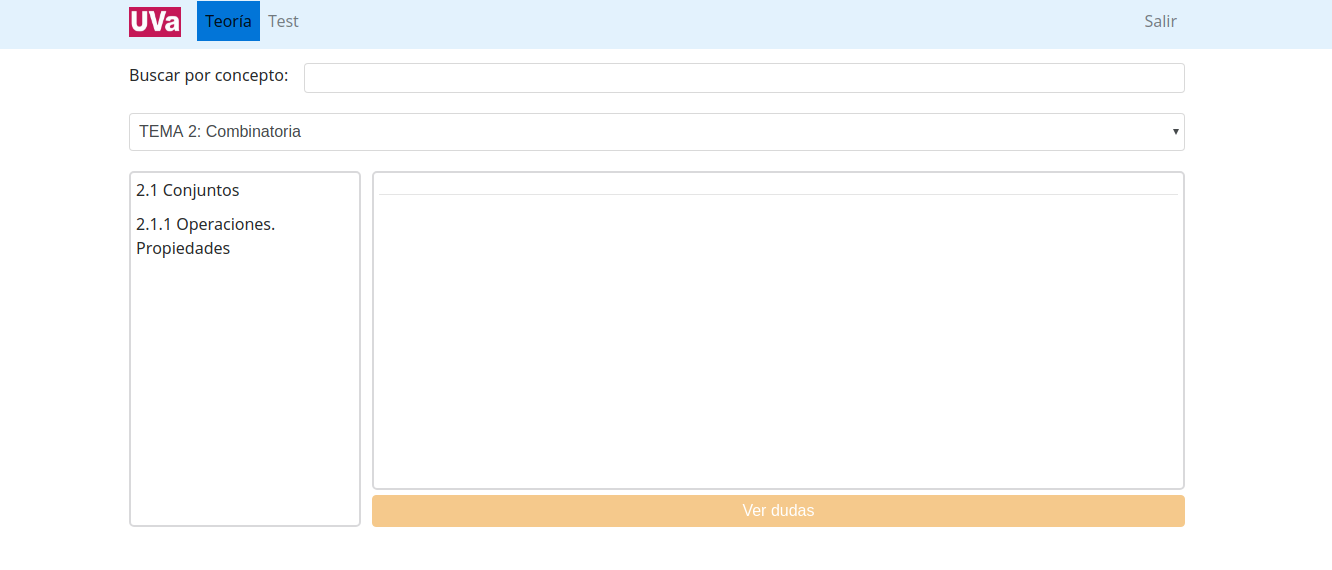
\includegraphics[width=\textwidth]{img/manual/alumno-teoria.png}
        \end{center}
        \caption{Pantalla inicial de teoría}
    \end{figure}
    
    Dentro de la pantalla de teoría se puede escoger un tema en el selector,
    y una vez seleccionado, se puede escoger un concepto. Tras clicar, se ve
    el contenido del concepto y las palabras relacionadas. A mayores, se
    activará el boton \enquote{Ver dudas}. También se puede buscar un
    concepto basándonos en sus palabras destacadas introduciendo la
    palabra(o parte de ella) en la barra de búsqueda de la parte superior.
    
    \begin{figure}[H]
        \begin{center}
            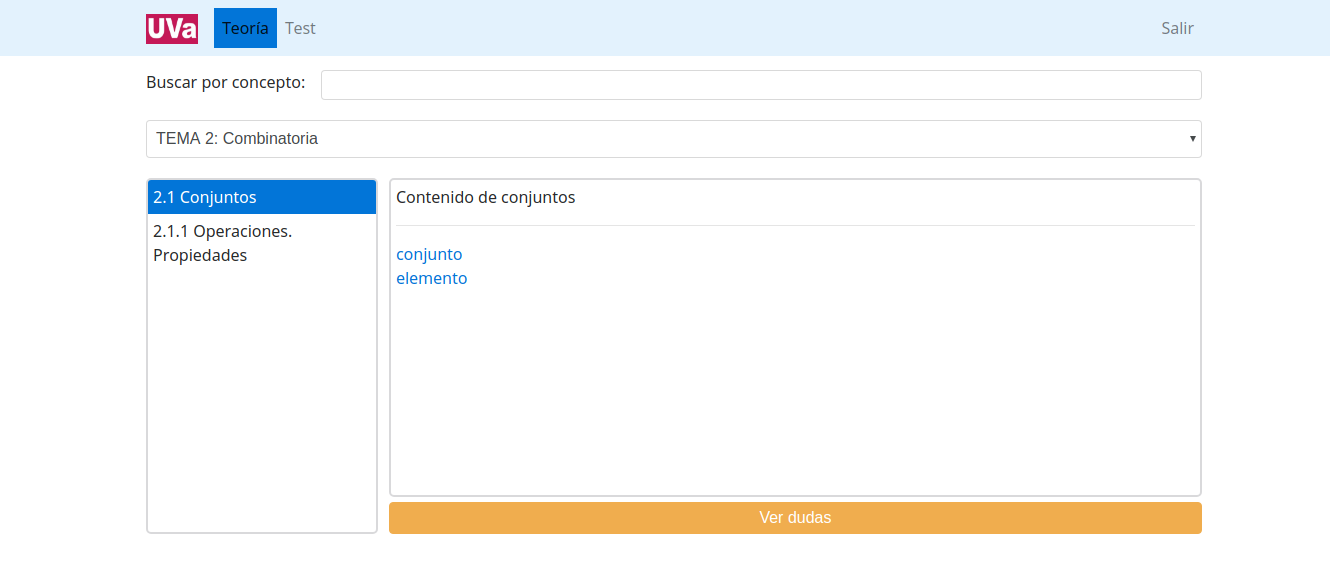
\includegraphics[width=\textwidth]{img/manual/alumno-teoria2.png}
        \end{center}
        \caption{Pantalla tras pulsar sobre un concepto}
    \end{figure}
    
    Pulsando en el botón \enquote{Ver dudas}, se accederá a la pantalla de
    dudas.
    
    \begin{figure}[H]
        \begin{center}
            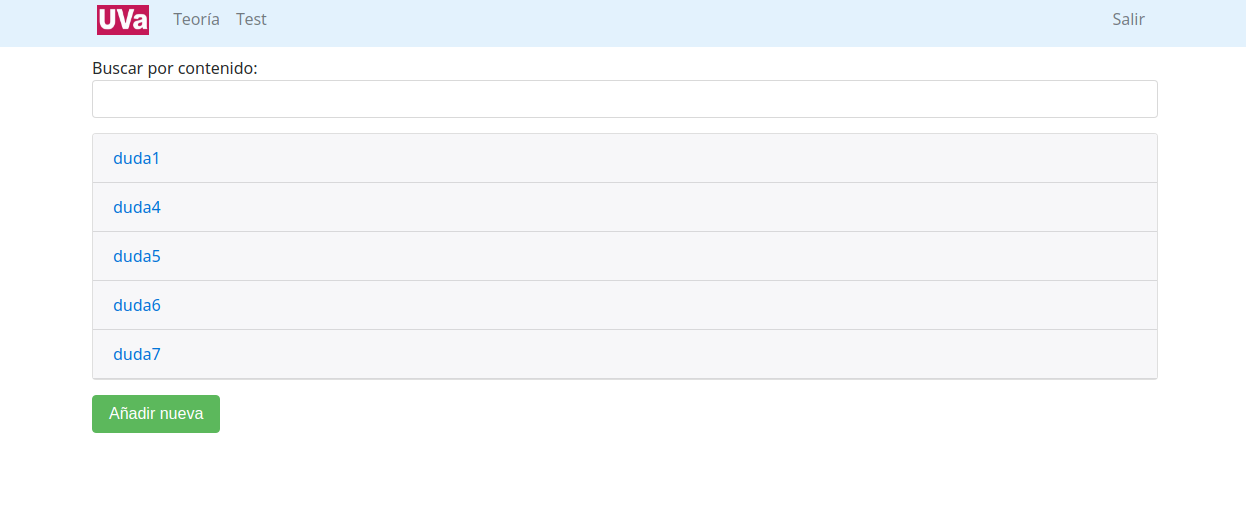
\includegraphics[width=\textwidth]{img/manual/alumno-teoria3.png}
        \end{center}
        \caption{Pantalla ver dudas}
    \end{figure}
    
    Al pulsar en una dudas se verá el contenido de la duda. Al pulsar sobre
    el boton \enquote{Añadir duda} se nos despliega un formulario que
    permite añadir los datos para insertar una nueva duda. Tras pulsar sobre
    el botón \enquote{Enviar} la aplicación redirige a una pantalla de
    confirmación. Finalmente, tras confirmar, la duda sera insertada. En
    esta pantalla también se puede ver una barra de búsqueda, que permite la
    búsqueda concreta de dudas en función de su contenido.
    
    Pulsando en el botón \enquote{Test} de la barra de navegación redirige a
    la pantalla principal de test.
    
    \begin{figure}[H]
        \begin{center}
            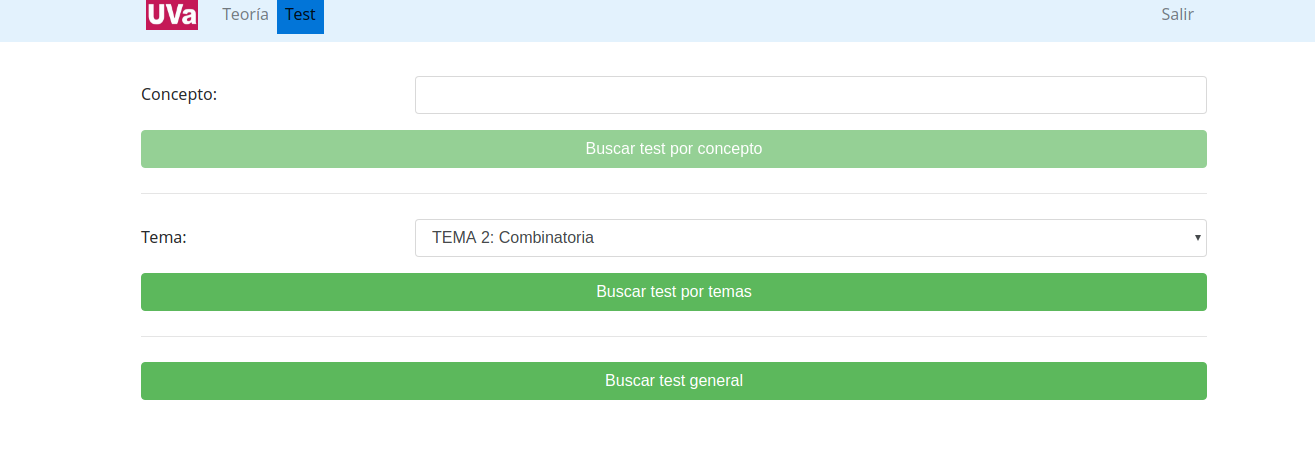
\includegraphics[width=\textwidth]{img/manual/alumno-test4.png}
        \end{center}
        \caption{Pantalla inicial de test}
    \end{figure}
    
    En este punto, se muestran 3 opciones, buscar test por concepto, buscar
    test por tema y buscar test general. Cada una de ellas generará un
    cuestionario basado en la opción escogida y redirigirá a una pantalla
    que permite rellenar el cuestionario.
    
    \begin{figure}[H]
        \begin{center}
            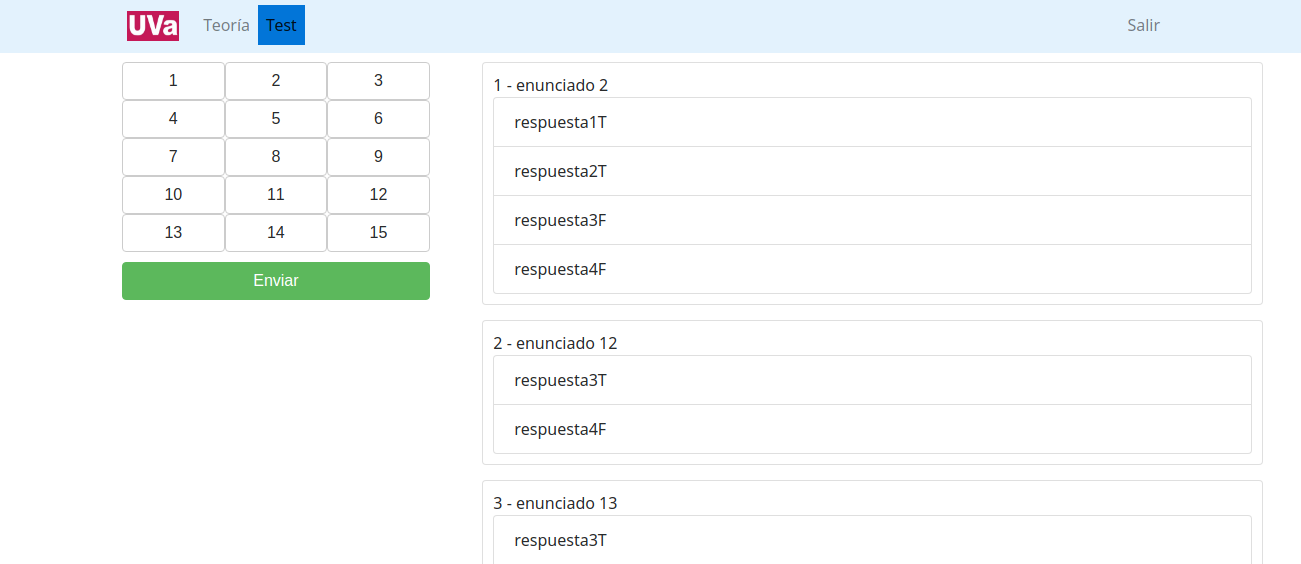
\includegraphics[width=\textwidth]{img/manual/alumno-test5.png}
        \end{center}
        \caption{Pantalla de cuestionario}
    \end{figure}
    
    Tras rellenarlo, se pulsa el botón \enquote{Enviar}y la aplicación
    redirigirá a una pantalla de confirmación. Tras confirmar, redigirá a
    una pantalla similar a la de cuestionario pero que incluye la resolución
    del mismo, así como la nota conseguida.
    
    \begin{figure}[H]
        \begin{center}
            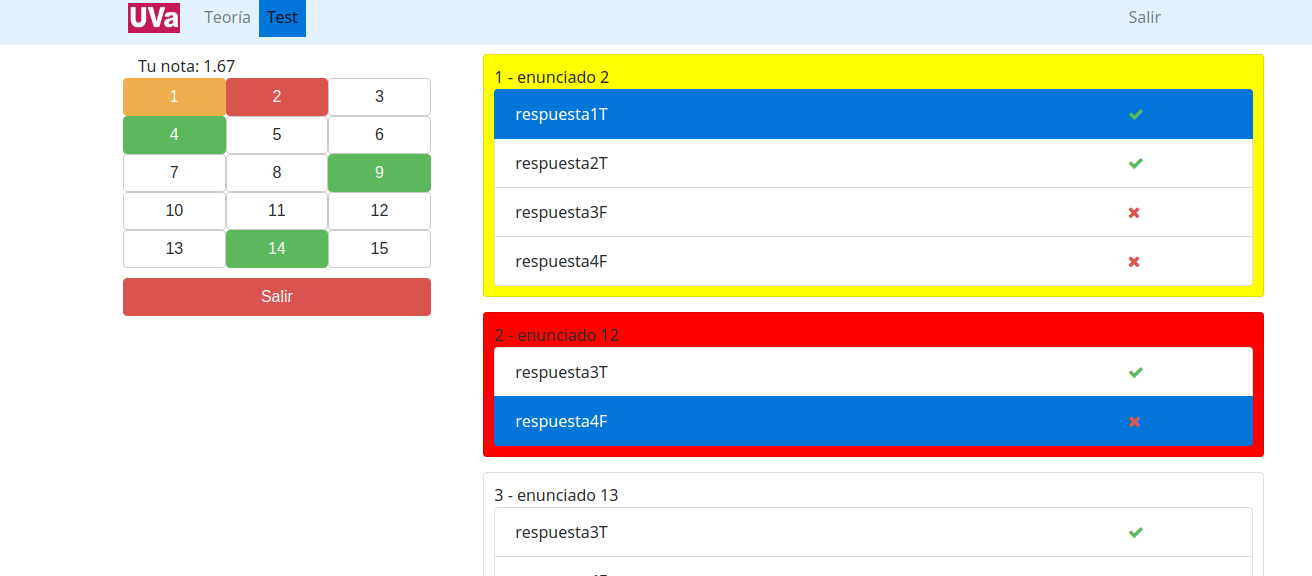
\includegraphics[width=\textwidth]{img/manual/alumno-test6.png}
        \end{center}
        \caption{Pantalla de resolución}
    \end{figure}
    
    \newpage
    
    \section{Manual del profesor:}\label{manual-del-profesor}
    
    Según se entra en la aplicación se accede a la pantalla de teoría. Se
    puede ver en la barra superior la barra de navegación, y en ella cuatro
    apartados, \enquote{Teoría}, \enquote{Dudas}, \enquote{Estadísticas} y
    \enquote{Test} y la opción \enquote{Salir}. Esta última opción, permite
    cerrar sesión. El apartado dudas, puede ir acompañado de un número, que
    indica el número de dudas sin resolver.
    
    \begin{figure}[H]
        \begin{center}
            \includegraphics[width=\textwidth]{img/manual/profesor-teoria.png}
        \end{center}
        \caption{Pantalla inicial de teoría del profesor}
    \end{figure}
    
    En esta pantalla se mantiene toda la funcionalidad explicada en el
    apartado \enquote{Manual del alumno}. Desde esta pantalla se permite
    añadir un nuevo elemento de teoría, pulsando en el botón
    \enquote{Añadir} y rellenando el formulario correspondiente. En el
    último paso, la aplicación pedirá confirmación para asegurar que los
    datos se han introducido correctamente.
    
    Volviendo a la pantalla inicial de teoría, tras pulsar en un concepto se
    permite borrarlo o editarlo pulsando los botones \enquote{Borrar} y
    \enquote{Editar} respectivamente. De forma análoga al paso de añadir
    tras finalizar el proceso, pedirá confirmación al usuario.
    
    La opción \enquote{Ver dudas}, funcionará de forma similar a la descrita
    en el apartado \enquote{Manual de alumno}, con el añadido de que, una
    vez seleccionadas, permite al profesor borrar dudas.
    
    Pulsando en el apartado \enquote{Dudas} de la barra de navegación la
    aplicación dirigirá a una nueva pantalla donde se muestran las nuevas
    dudas sin resolver. Tras pulsar sobre una de ellas, se muestra el
    contenido, el concepto relacionado y tres opciones, \enquote{Reportar},
    \enquote{Ignorar por repetido}, \enquote{Responder}. \enquote{Reportar}
    significa que la duda es inapropiada u ofensiva. \enquote{Ignorar por
    repetido} significa que la dudas está repetida y que no va a ser
    respondida. Por último, la opción \enquote{Responder} permite al
    profesor responder la duda. El sistema pedirá confirmación antes de
    hacer cualquiera de estas acciones, ya sea mediante un aviso en el caso
    de \enquote{Reportar} e \enquote{Ignorar} o mediante una pantalla de
    confirmación en el caso de ``Responder.
    
    \begin{figure}[H]
        \begin{center}
            \includegraphics[width=\textwidth]{img/manual/profesor-dudas.png}
        \end{center}
        \caption{Pantalla de dudas}
    \end{figure}
    
    La opción \enquote{Test} de la barra de navegación redirige a la
    pantalla de test.
    
    \begin{figure}[H]
        \begin{center}
            \includegraphics[width=\textwidth]{img/manual/profesor-test.png}
        \end{center}
        \caption{Pantalla inicial de test del profesor}
    \end{figure}
    
    En ella, el profesor escoge un tema y pulsa el botón \enquote{Revisar}.
    Tras ello, se muestran los enunciados de las cuestiones y el botón
    \enquote{Añadir}.
    
    \begin{figure}[H]
        \begin{center}
            \includegraphics[width=\textwidth]{img/manual/profesor-test2.png}
        \end{center}
        \caption{Pantalla de test del profesor}
    \end{figure}
    
    Pulsando sobre cualquiera de ellos, se mostrarán las posibles
    respuestas, marcando con un tick las correctas y los botones
    \enquote{Editar} y \enquote{Borrar}. Si se escoge la opción borrar, la
    aplicación pedirá al profesor confirmación antes de borrarla. Pulsando
    sobre \enquote{Confirmar} la cuestión será eliminada. Si se escoge la
    opción \enquote{Editar}, la aplicación nos redirigirá a una pantalla en
    la cual podremos modificar el contenido de la cuestión. El formulario de
    editar funciona de manera análoga a la opción añadir, que será explicada
    a continuación. Finalmente, tras confirmar, la cuestion será editada.
    
    \begin{figure}[H]
        \begin{center}
            \includegraphics[width=\textwidth]{img/manual/profesor-test2-desplegada.png}
        \end{center}
        \caption{Pantalla de test del profesor con duda desplegada}
    \end{figure}
    
    La opción \enquote{Añadir} permite al profesor añadir una nueva
    cuestión. Al pulsarla, nos redirigirá a la siguiente pantalla.
    
    \begin{figure}[H]
        \begin{center}
            \includegraphics[width=\textwidth]{img/manual/profesor-test3-aniadir.png}
        \end{center}
        \caption{Pantalla de añadir pregunta}
    \end{figure}
    
    Esta pantalla muestra un formulario que formará la pregunta. Para añadir
    nuevas opciones es necesario que todas las opciones incluidas sean
    válidas, es decir, no estén vacías ni sean repetidas. En la foto
    anterior se puede observar que, al estar vacía no permite añadir nuevas
    opciones. Tras rellenar el campo opción, se puede elegir si la respuesta
    es correcta o incorrecta cambiando el símbolo a la derecha clicando.
    
    \begin{figure}[H]
        \begin{center}
            \includegraphics[width=\textwidth]{img/manual/opcion-verdadera.png}
        \end{center}
        \caption{Pantalla de opción verdadera}
    \end{figure}
    
    \begin{figure}[H]
        \begin{center}
            \includegraphics[width=\textwidth]{img/manual/opcion-falsa.png}
        \end{center}
        \caption{Pantalla de opción falsa}
    \end{figure}
    
    Tras tener una serie de respuestas que cumplan con las condiciones
    necesarias, esto es, que no tengan opciones repetidas ni vacías y que al
    menos una de ellas sea verdadera y una falsa; pulsando en el botón
    \enquote{Añadir}, la aplicación pedirá confirmación, y tras confirmar,
    la cuestión será guardada.
    
    Por último, el apartado \enquote{Estadísticas} de la barra superior nos
    redigirá a la página de estadísticas.
    
    \begin{figure}[H]
        \begin{center}
            \includegraphics[width=\textwidth]{img/manual/profesor-estadisticas.png}
        \end{center}
        \caption{Pantalla de principal de estadísticas}
    \end{figure}
    
    En ella, el profesor introduce un nombre de alumno y la aplicación
    muestra el número de conceptos visitados, el número de cuestionarios
    realizados y el número de dudas preguntadas.
    
    \begin{figure}[H]
        \begin{center}
            \includegraphics[width=\textwidth]{img/manual/profesor-estadisticas2.png}
        \end{center}
        \caption{Pantalla de estadísticas tras buscar}
    \end{figure}
    
    Al pulsar sobre cada uno de estos recuadros, se obtendrá información en
    detalle.
    
    \begin{figure}[H]
        \begin{center}
            \includegraphics[width=\textwidth]{img/manual/profesor-estadisticas-detalle1.png}
        \end{center}
        \caption{Pantalla de detalle de los conceptos visitados}
    \end{figure}
    
    Destacar del detalle de las dudas planteadas que marca en rojo las
    previamente reportadas por el profesor y en naranja las proviamente
    ignoradas.
    
    \begin{figure}[H]
        \begin{center}
            \includegraphics[width=\textwidth]{img/manual/profesor-estadisticas-detalle2.png}
        \end{center}
        \caption{Pantalla de detalle de las dudas planteadas}
    \end{figure}
    
    Destacar del detalle de los cuestionario realizados que marca en rojo
    los cuestionarios suspensos y en verde los cuestionarios aprobados. Al
    pulsar el botón \enquote{Ver cuestionario}, redigirá a una página que
    mostrará el cuestionario tal y como lo vio el alumno en su corrección.
    
    \begin{figure}[H]
        \begin{center}
            \includegraphics[width=\textwidth]{img/manual/profesor-estadisticas-detalle3.png}
        \end{center}
        \caption{Pantalla de detalle de los cuestionarios realizados}
    \end{figure}
    
    \chapter{Contenido del CD-ROM}\label{contenido-del-cd-rom}
    
    El CD incluye los ficheros generados durante la elaboración del trabajo.
    Éste se divide en tres directorios que describiremos a continuación:
    
    \section{Directorio Documentation}\label{directorio-documentation}
    
    Este es el directorio que contiene los ficheros fuente de la elaboración
    de esta memoria. El contenido se encuentra en formato markdown dividido
    en secciones en la carpeta secciones. En la carpeta latex podemos ver
    algunos ficheros necesarios para la creación del documento final. La
    carpeta img almacena categorizados en subcarpetas las imágenes que
    después se referencian desde el documento. También están en esa carpeta
    algunos diagramas creados. En la raiz del directorio está el fichero
    bibliografia.bib, con la información bibliográfica en formato BibTeX y
    el fichero main.mdpp que define la estructura del documento y algunos
    metadatos como el título, agradecimiento y autor.
    
    \section{Directorio backend}\label{directorio-backend}
    
    En este directorio encontramos los ficheros relacionados con el código
    fuente del backend de la aplicación, así como los ficheros de
    configuración.
    
    \section{Directorio frontend}\label{directorio-frontend}
    
    En este directorio encontramos los ficheros relacionados con el código
    fuente del frontend de la aplicación, así como los ficheros de
    configuración.
    
    \addcontentsline{toc}{chapter}{Bibliografía}
    
    \nocite{*} \printbibliography

    \cleardoublepage
    %\renewcommand\bibname{Referencias Web}

    %\begin{thebibliography}{X}
    %    \bibitem{ref1} \textit{Ejemplo}, \\
    %    \textsc{ejemplo.com}.
    %    \\Recuperado a tal fecha, \\de \href{http://ejemplo.com}
    %\end{thebibliography}
\end{document}